\documentclass[aspectratio=169,10pt]{beamer}

% Modern professional theme for computer vision presentation
\usetheme{metropolis}
\usecolortheme{default}

% Custom color scheme optimized for computer vision presentation
\definecolor{primaryblue}{RGB}{20,75,140}
\definecolor{secondaryblue}{RGB}{70,130,180}
\definecolor{accentorange}{RGB}{230,95,45}
\definecolor{lightgray}{RGB}{245,245,245}
\definecolor{darkgray}{RGB}{45,45,45}

% Metropolis color customization
\setbeamercolor{progress bar}{fg=primaryblue,bg=lightgray}
\setbeamercolor{title separator}{fg=primaryblue}
\setbeamercolor{progress bar in head/foot}{fg=primaryblue}
\setbeamercolor{progress bar in section page}{fg=primaryblue}
\setbeamercolor{frametitle}{bg=primaryblue,fg=white}
\setbeamercolor{title}{fg=primaryblue}
\setbeamercolor{subtitle}{fg=secondaryblue}
\setbeamercolor{structure}{fg=primaryblue}
\setbeamercolor{alerted text}{fg=accentorange}
\setbeamercolor{block title}{bg=primaryblue,fg=white}
\setbeamercolor{block body}{bg=lightgray,fg=darkgray}
\setbeamercolor{block title alerted}{bg=accentorange,fg=white}
\setbeamercolor{block body alerted}{bg=lightgray,fg=darkgray}

% Enhanced packages for mathematical rigor
\usepackage{amsmath,amssymb,amsfonts}
\usepackage{graphicx}
\usepackage{booktabs}
\usepackage{xcolor}
\usepackage{tikz}
\usepackage{algorithm2e}

% Professional formatting
\setbeamertemplate{navigation symbols}{}
\setbeamertemplate{footline}[frame number]

% Title information
\title{Image Segmentation and Morphological Processing}
\subtitle{CMSC 178IP - Digital Image Processing}
\author{Noel Jeffrey Pinton}
\institute{University of the Philippines - Cebu\\Department of Computer Science}
\date{}

\begin{document}

% Title slide
\begin{frame}
\titlepage
\end{frame}

% Table of contents
\begin{frame}{Course Outline}
\tableofcontents
\end{frame}

\section{Introduction to Image Segmentation}

\begin{frame}{What is Image Segmentation?}
\begin{alertblock}{Definition}
Image segmentation is the process of partitioning an image into multiple segments or regions to simplify representation and make it more meaningful for analysis.
\end{alertblock}

\textbf{Goal:} Group pixels into regions based on:
\begin{itemize}
\item Intensity similarity
\item Spatial proximity
\item Texture patterns
\item Color characteristics
\end{itemize}

\vspace{0.3cm}
\textbf{Applications:}
Medical imaging, autonomous vehicles, object recognition, satellite imagery
\end{frame}

\begin{frame}{Segmentation Challenges}
\begin{columns}
\column{0.5\textwidth}
\textbf{Key Challenges:}
\begin{itemize}
\item Varying illumination
\item Object occlusion
\item Noise and artifacts
\item Ambiguous boundaries
\item Scale variations
\item Texture complexity
\end{itemize}

\column{0.5\textwidth}
\begin{block}{Success Criteria}
\begin{itemize}
\item Regions should be uniform
\item Adjacent regions differ significantly
\item Region interiors are simple
\item Boundaries are smooth and accurate
\end{itemize}
\end{block}
\end{columns}
\end{frame}

\section{Thresholding Methods}

\begin{frame}{Global Thresholding}
\textbf{Simplest segmentation approach:} Partition image based on intensity threshold

\textbf{Binary segmentation:}
$$g(x,y) = \begin{cases}
1 & \text{if } f(x,y) > T \\
0 & \text{if } f(x,y) \leq T
\end{cases}$$

\textbf{Advantages:}
\begin{itemize}
\item Simple and fast computation
\item Effective for bimodal histograms
\item Low memory requirements
\end{itemize}

\textbf{Limitations:}
\begin{itemize}
\item Fails with varying illumination
\item Sensitive to noise
\item Requires manual threshold selection
\end{itemize}
\end{frame}

\begin{frame}{Global Thresholding: Visual Example}
\begin{center}
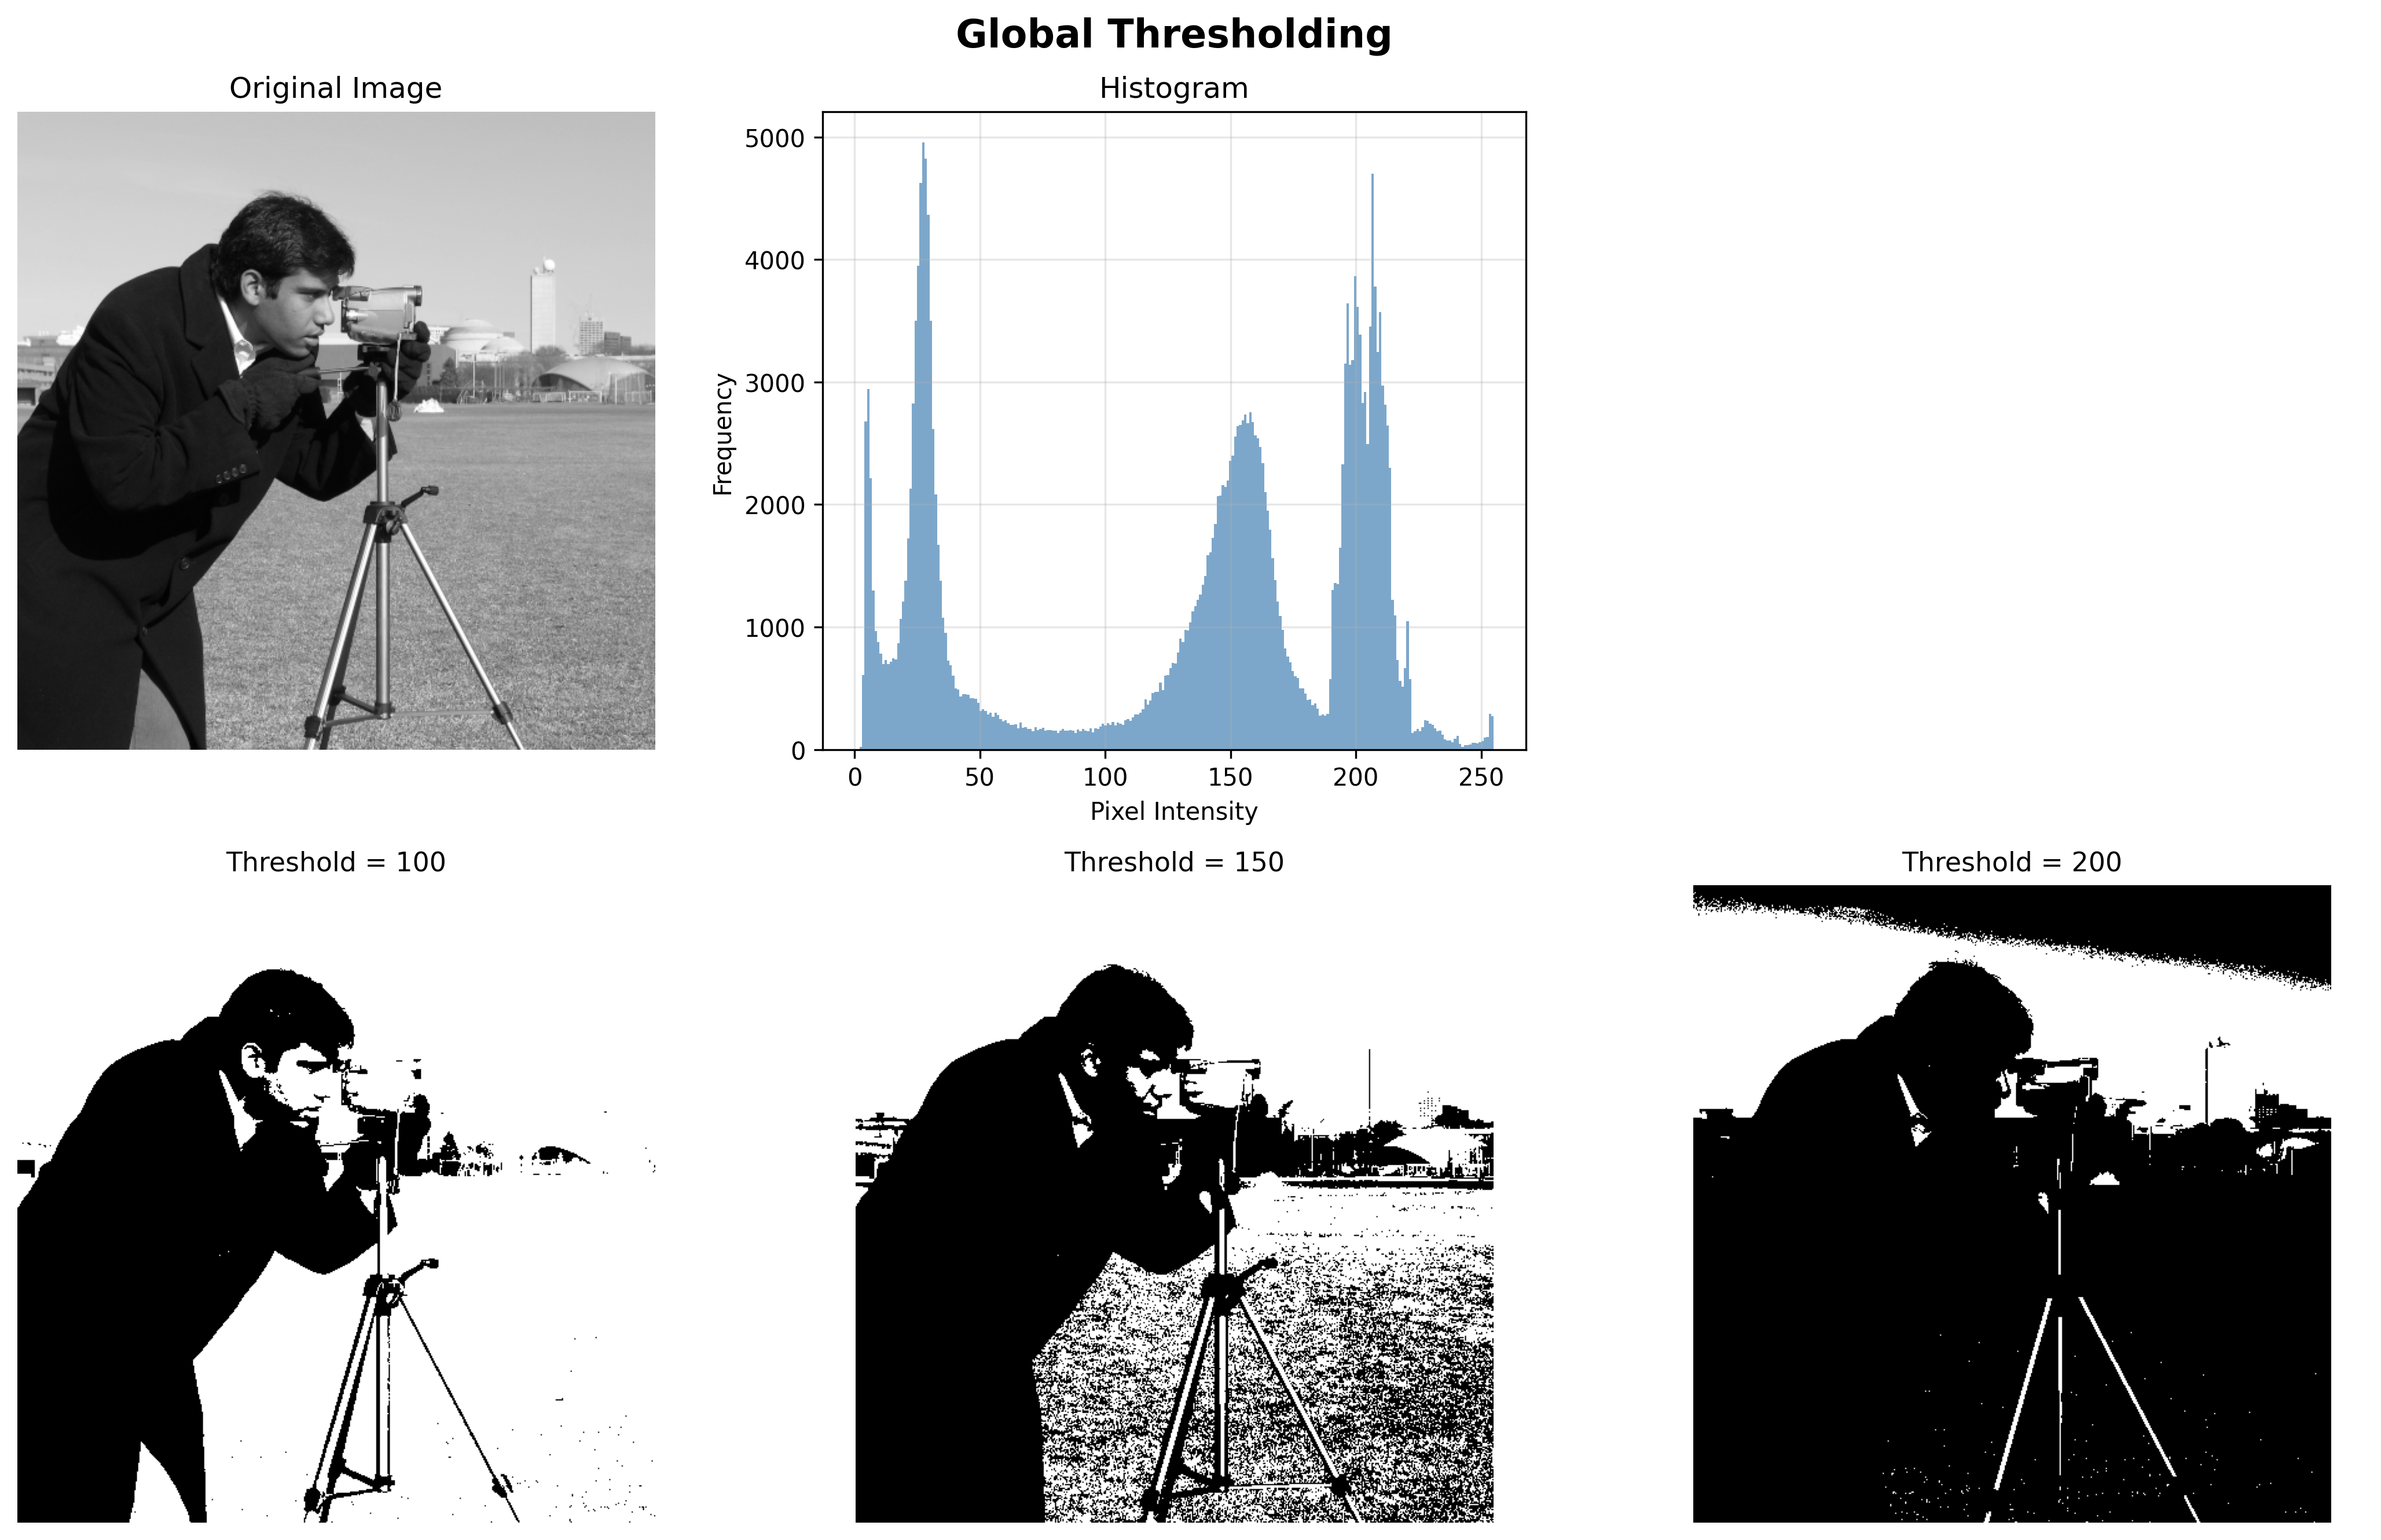
\includegraphics[width=0.95\textwidth,height=0.75\textheight,keepaspectratio]{../figures/01_global_thresholding.png}
\end{center}
\end{frame}

\begin{frame}{Otsu's Method}
\begin{alertblock}{Key Idea}
Automatically determine optimal threshold by maximizing between-class variance (equivalently, minimizing within-class variance).
\end{alertblock}

\textbf{Algorithm:}
For threshold $t$, compute:
$$\sigma_B^2(t) = \omega_0(t) \sigma_0^2(t) + \omega_1(t) \sigma_1^2(t)$$

Where:
\begin{itemize}
\item $\omega_0, \omega_1$ = class probabilities
\item $\sigma_0^2, \sigma_1^2$ = class variances
\item Optimal $t^* = \arg\max_t \sigma_B^2(t)$
\end{itemize}
\end{frame}

\begin{frame}{Otsu's Method: Implementation}
\textbf{Between-class variance:}
$$\sigma_B^2(t) = \omega_0(t) \omega_1(t) [\mu_0(t) - \mu_1(t)]^2$$

\textbf{Class probabilities:}
$$\omega_0(t) = \sum_{i=0}^{t} p_i, \quad \omega_1(t) = \sum_{i=t+1}^{L-1} p_i$$

\textbf{Class means:}
$$\mu_0(t) = \frac{1}{\omega_0} \sum_{i=0}^{t} i \cdot p_i, \quad \mu_1(t) = \frac{1}{\omega_1} \sum_{i=t+1}^{L-1} i \cdot p_i$$

where $p_i$ is the normalized histogram at intensity $i$
\end{frame}

\begin{frame}{Otsu's Method: Results}
\begin{center}
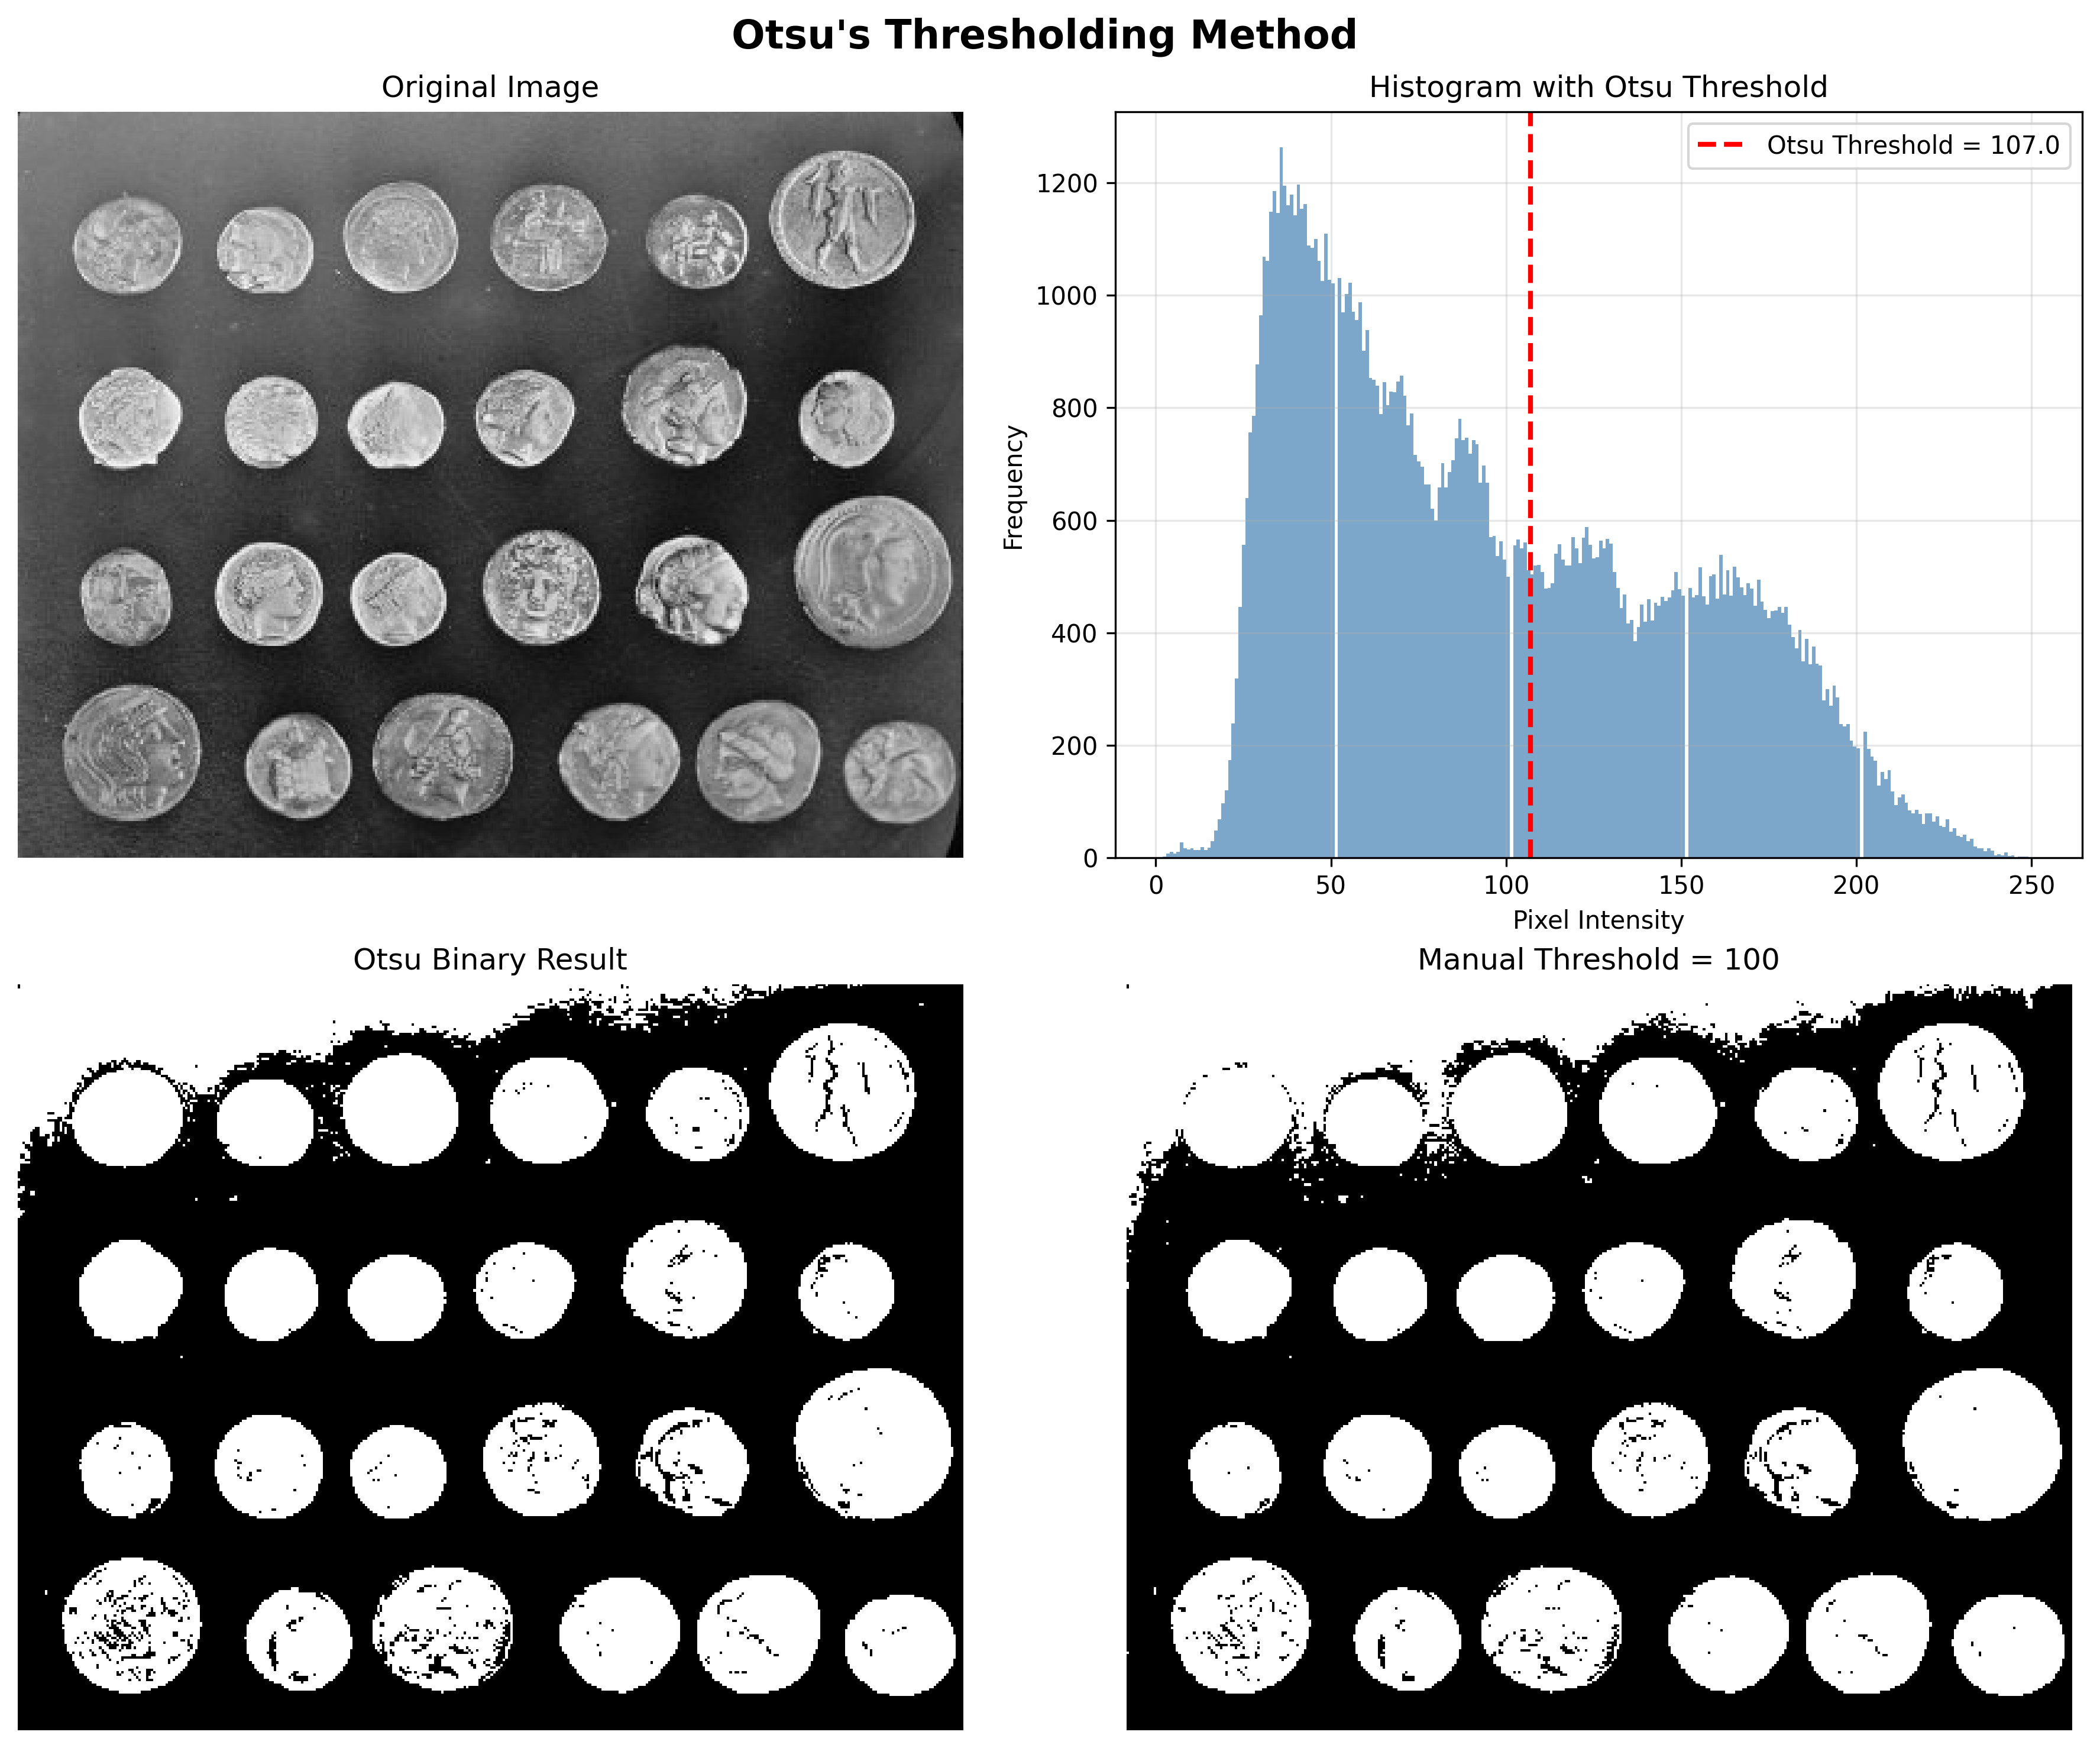
\includegraphics[width=0.88\textwidth,height=0.7\textheight,keepaspectratio]{../figures/02_otsu_thresholding.png}
\end{center}
\end{frame}

\begin{frame}{Local (Adaptive) Thresholding}
\textbf{Motivation:} Global methods fail with non-uniform illumination

\textbf{Approach:} Compute threshold locally in neighborhoods

$$T(x,y) = \text{function}(\text{local neighborhood around } (x,y))$$

\textbf{Common methods:}
\begin{itemize}
\item Mean of local region: $T(x,y) = \mu(x,y) - C$
\item Median of local region: $T(x,y) = \text{median}(N_{x,y}) - C$
\item Gaussian-weighted mean
\end{itemize}

where $C$ is a constant offset and $N_{x,y}$ is the local neighborhood
\end{frame}

\begin{frame}{Local Thresholding: Visual Comparison}
\begin{center}
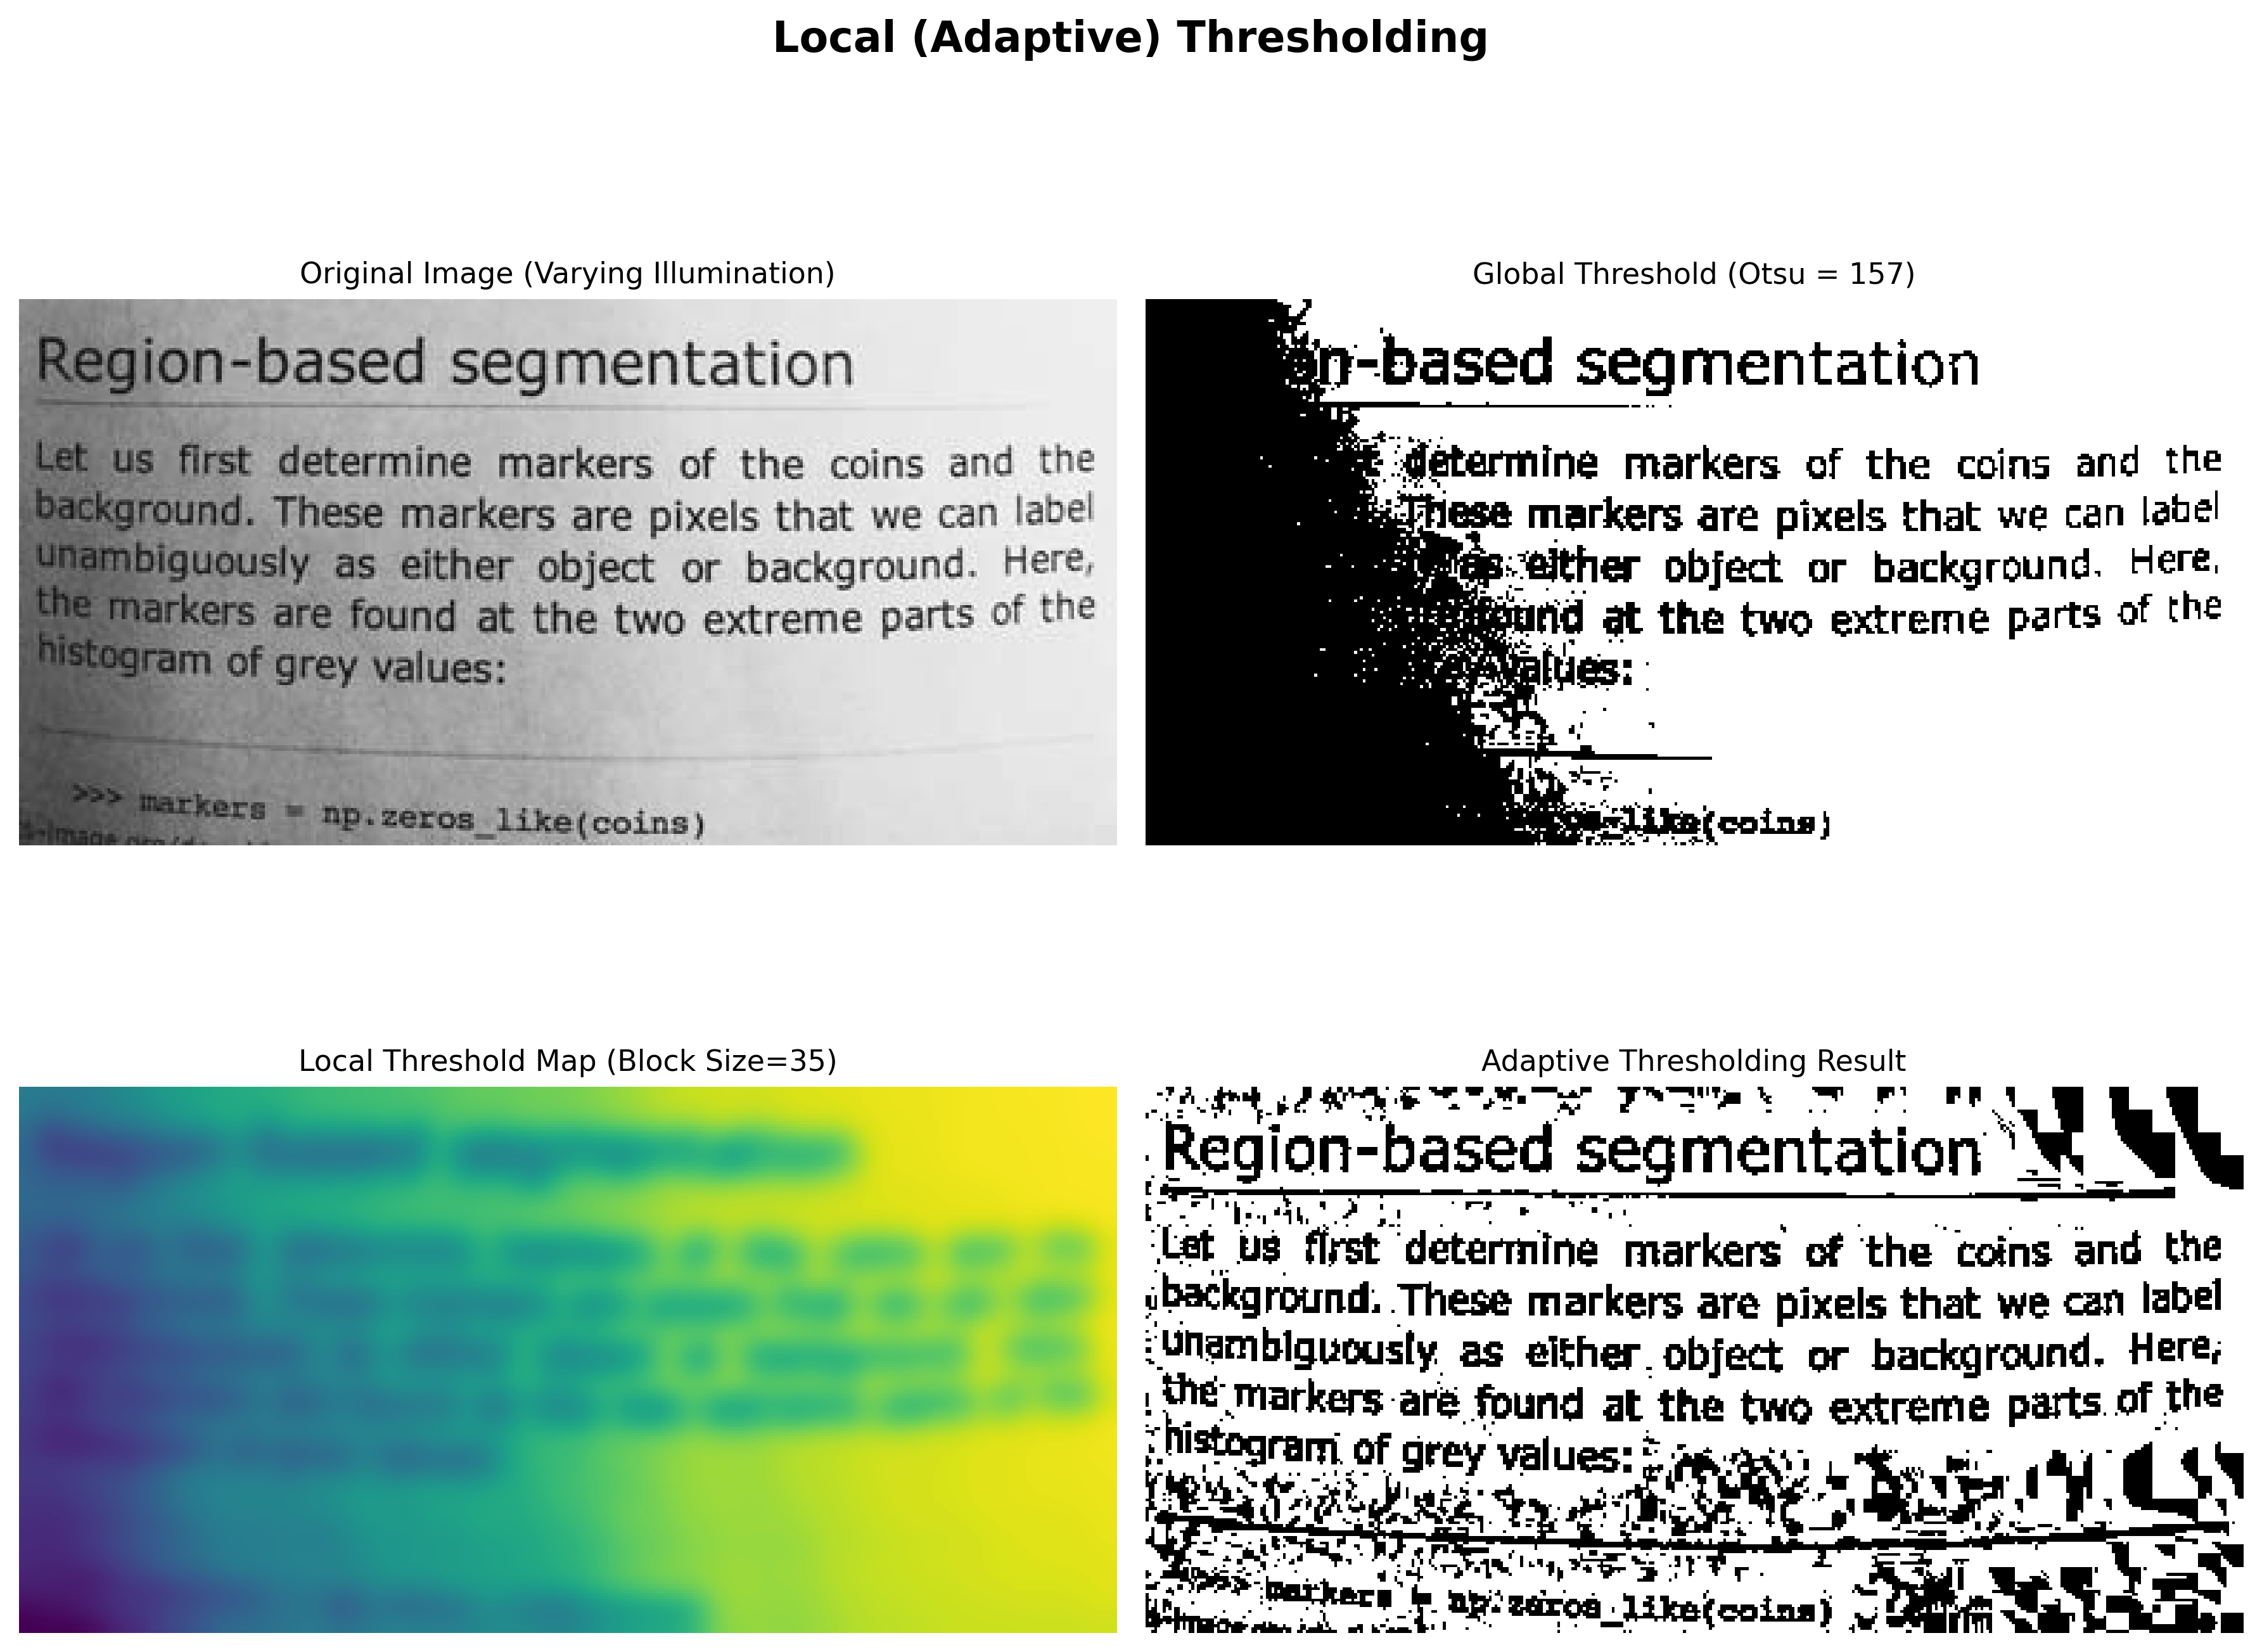
\includegraphics[width=0.92\textwidth,height=0.72\textheight,keepaspectratio]{../figures/03_local_thresholding.png}
\end{center}
\end{frame}

\section{Region-Based Segmentation}

\begin{frame}{Region Growing}
\begin{alertblock}{Concept}
Start from seed points and iteratively add neighboring pixels that satisfy similarity criteria.
\end{alertblock}

\textbf{Algorithm:}
\begin{enumerate}
\item Select seed point(s) $S = \{(x_0, y_0)\}$
\item Define similarity criterion $P(x,y)$
\item For each pixel in neighborhood:
\begin{itemize}
\item If $|f(x,y) - \mu_R| < T$, add to region
\item Update region statistics $\mu_R$
\end{itemize}
\item Repeat until no pixels can be added
\end{enumerate}

\textbf{Similarity criteria:} Intensity difference, gradient, texture, color
\end{frame}

\begin{frame}{Region Growing: Characteristics}
\textbf{Advantages:}
\begin{itemize}
\item Produces connected regions
\item Can incorporate spatial information
\item Flexible similarity criteria
\item Good for well-defined objects
\end{itemize}

\textbf{Disadvantages:}
\begin{itemize}
\item Sensitive to seed selection
\item Computationally expensive
\item May leak into adjacent regions
\item Requires threshold tuning
\end{itemize}
\end{frame}

\begin{frame}{Region Growing: Example}
\begin{center}
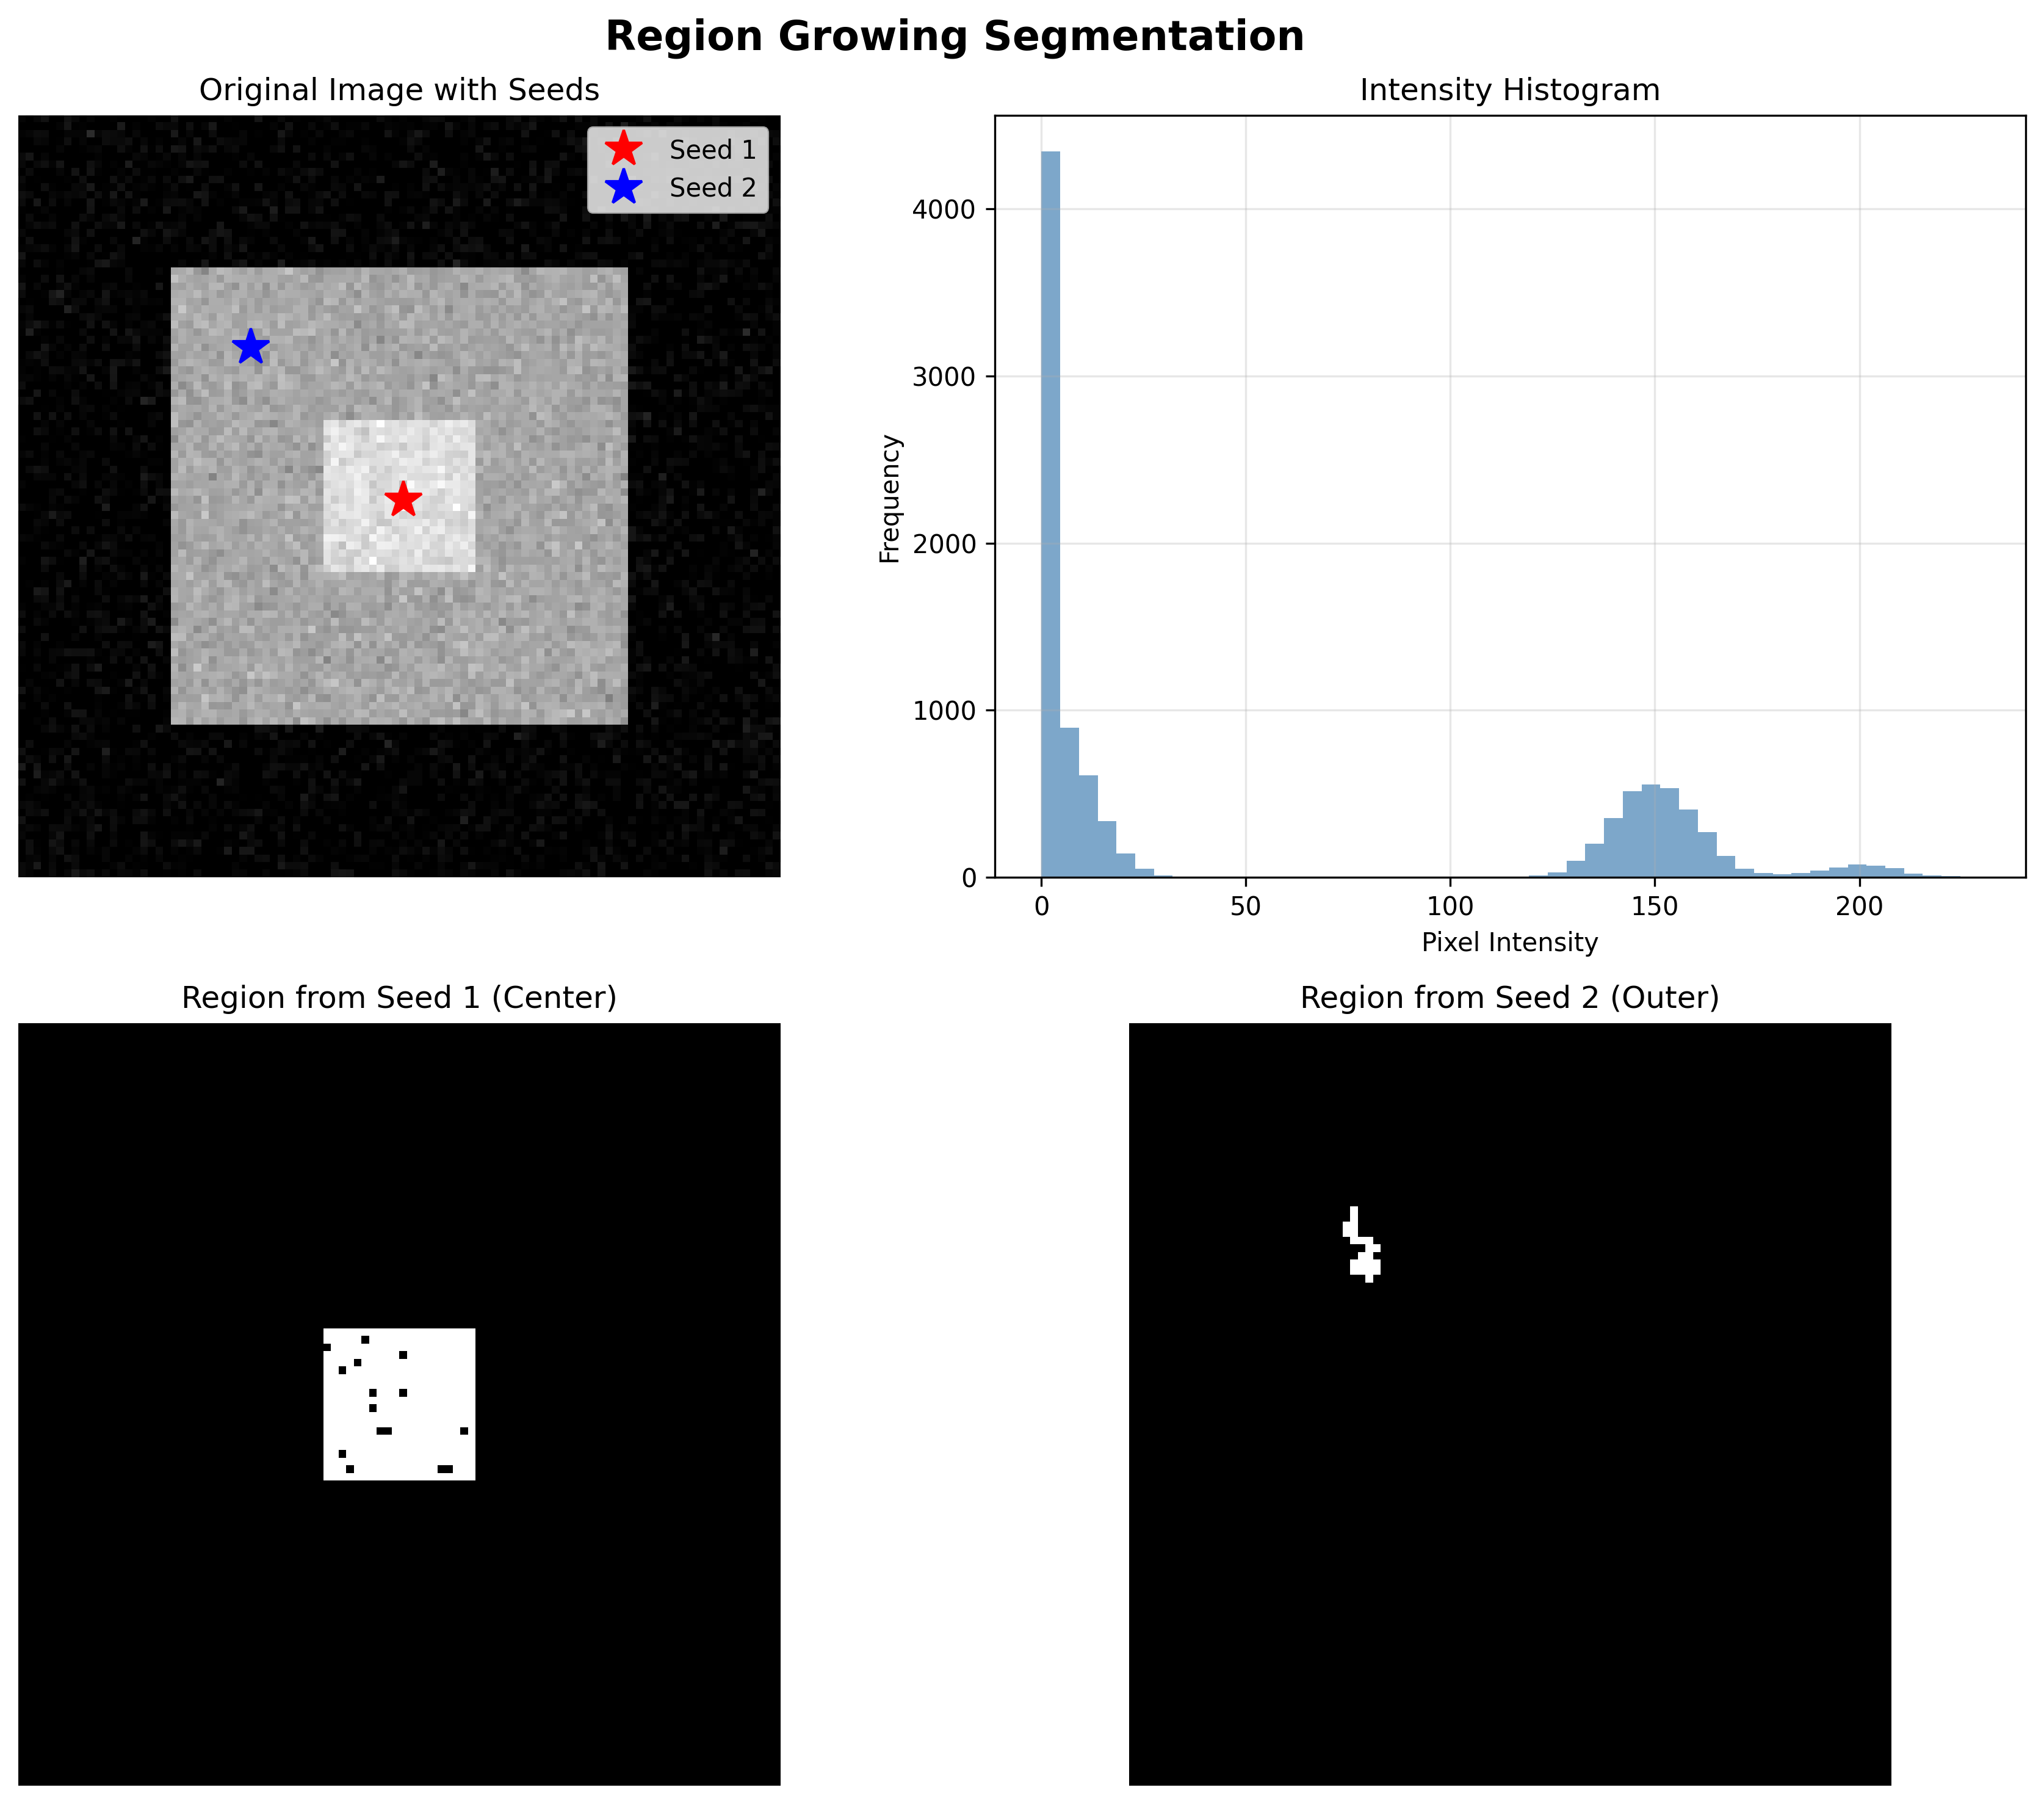
\includegraphics[width=0.85\textwidth,height=0.68\textheight,keepaspectratio]{../figures/04_region_growing.png}
\end{center}
\end{frame}

\begin{frame}{Watershed Segmentation}
\begin{alertblock}{Intuition}
Treat image as topographic surface where intensity represents elevation. Fill basins from local minima to create watershed lines.
\end{alertblock}

\textbf{Topographic interpretation:}
\begin{itemize}
\item Regional minima: catchment basins
\item Gradient magnitude: elevation
\item Watershed lines: region boundaries
\end{itemize}

\textbf{Key challenge:} Over-segmentation due to noise
\textbf{Solution:} Marker-controlled watershed
\end{frame}

\begin{frame}{Watershed Algorithm}
\textbf{Steps:}
\begin{enumerate}
\item Compute gradient magnitude: $\nabla f = \sqrt{(\frac{\partial f}{\partial x})^2 + (\frac{\partial f}{\partial y})^2}$
\item Find regional minima (markers)
\item Simulate flooding from minima
\item Build dams (watershed lines) where waters meet
\end{enumerate}

\textbf{Marker-controlled approach:}
\begin{itemize}
\item Use distance transform for internal markers
\item Apply morphological operations to reduce over-segmentation
\item Merge regions based on similarity
\end{itemize}
\end{frame}

\begin{frame}{Watershed Segmentation: Pipeline}
\begin{center}
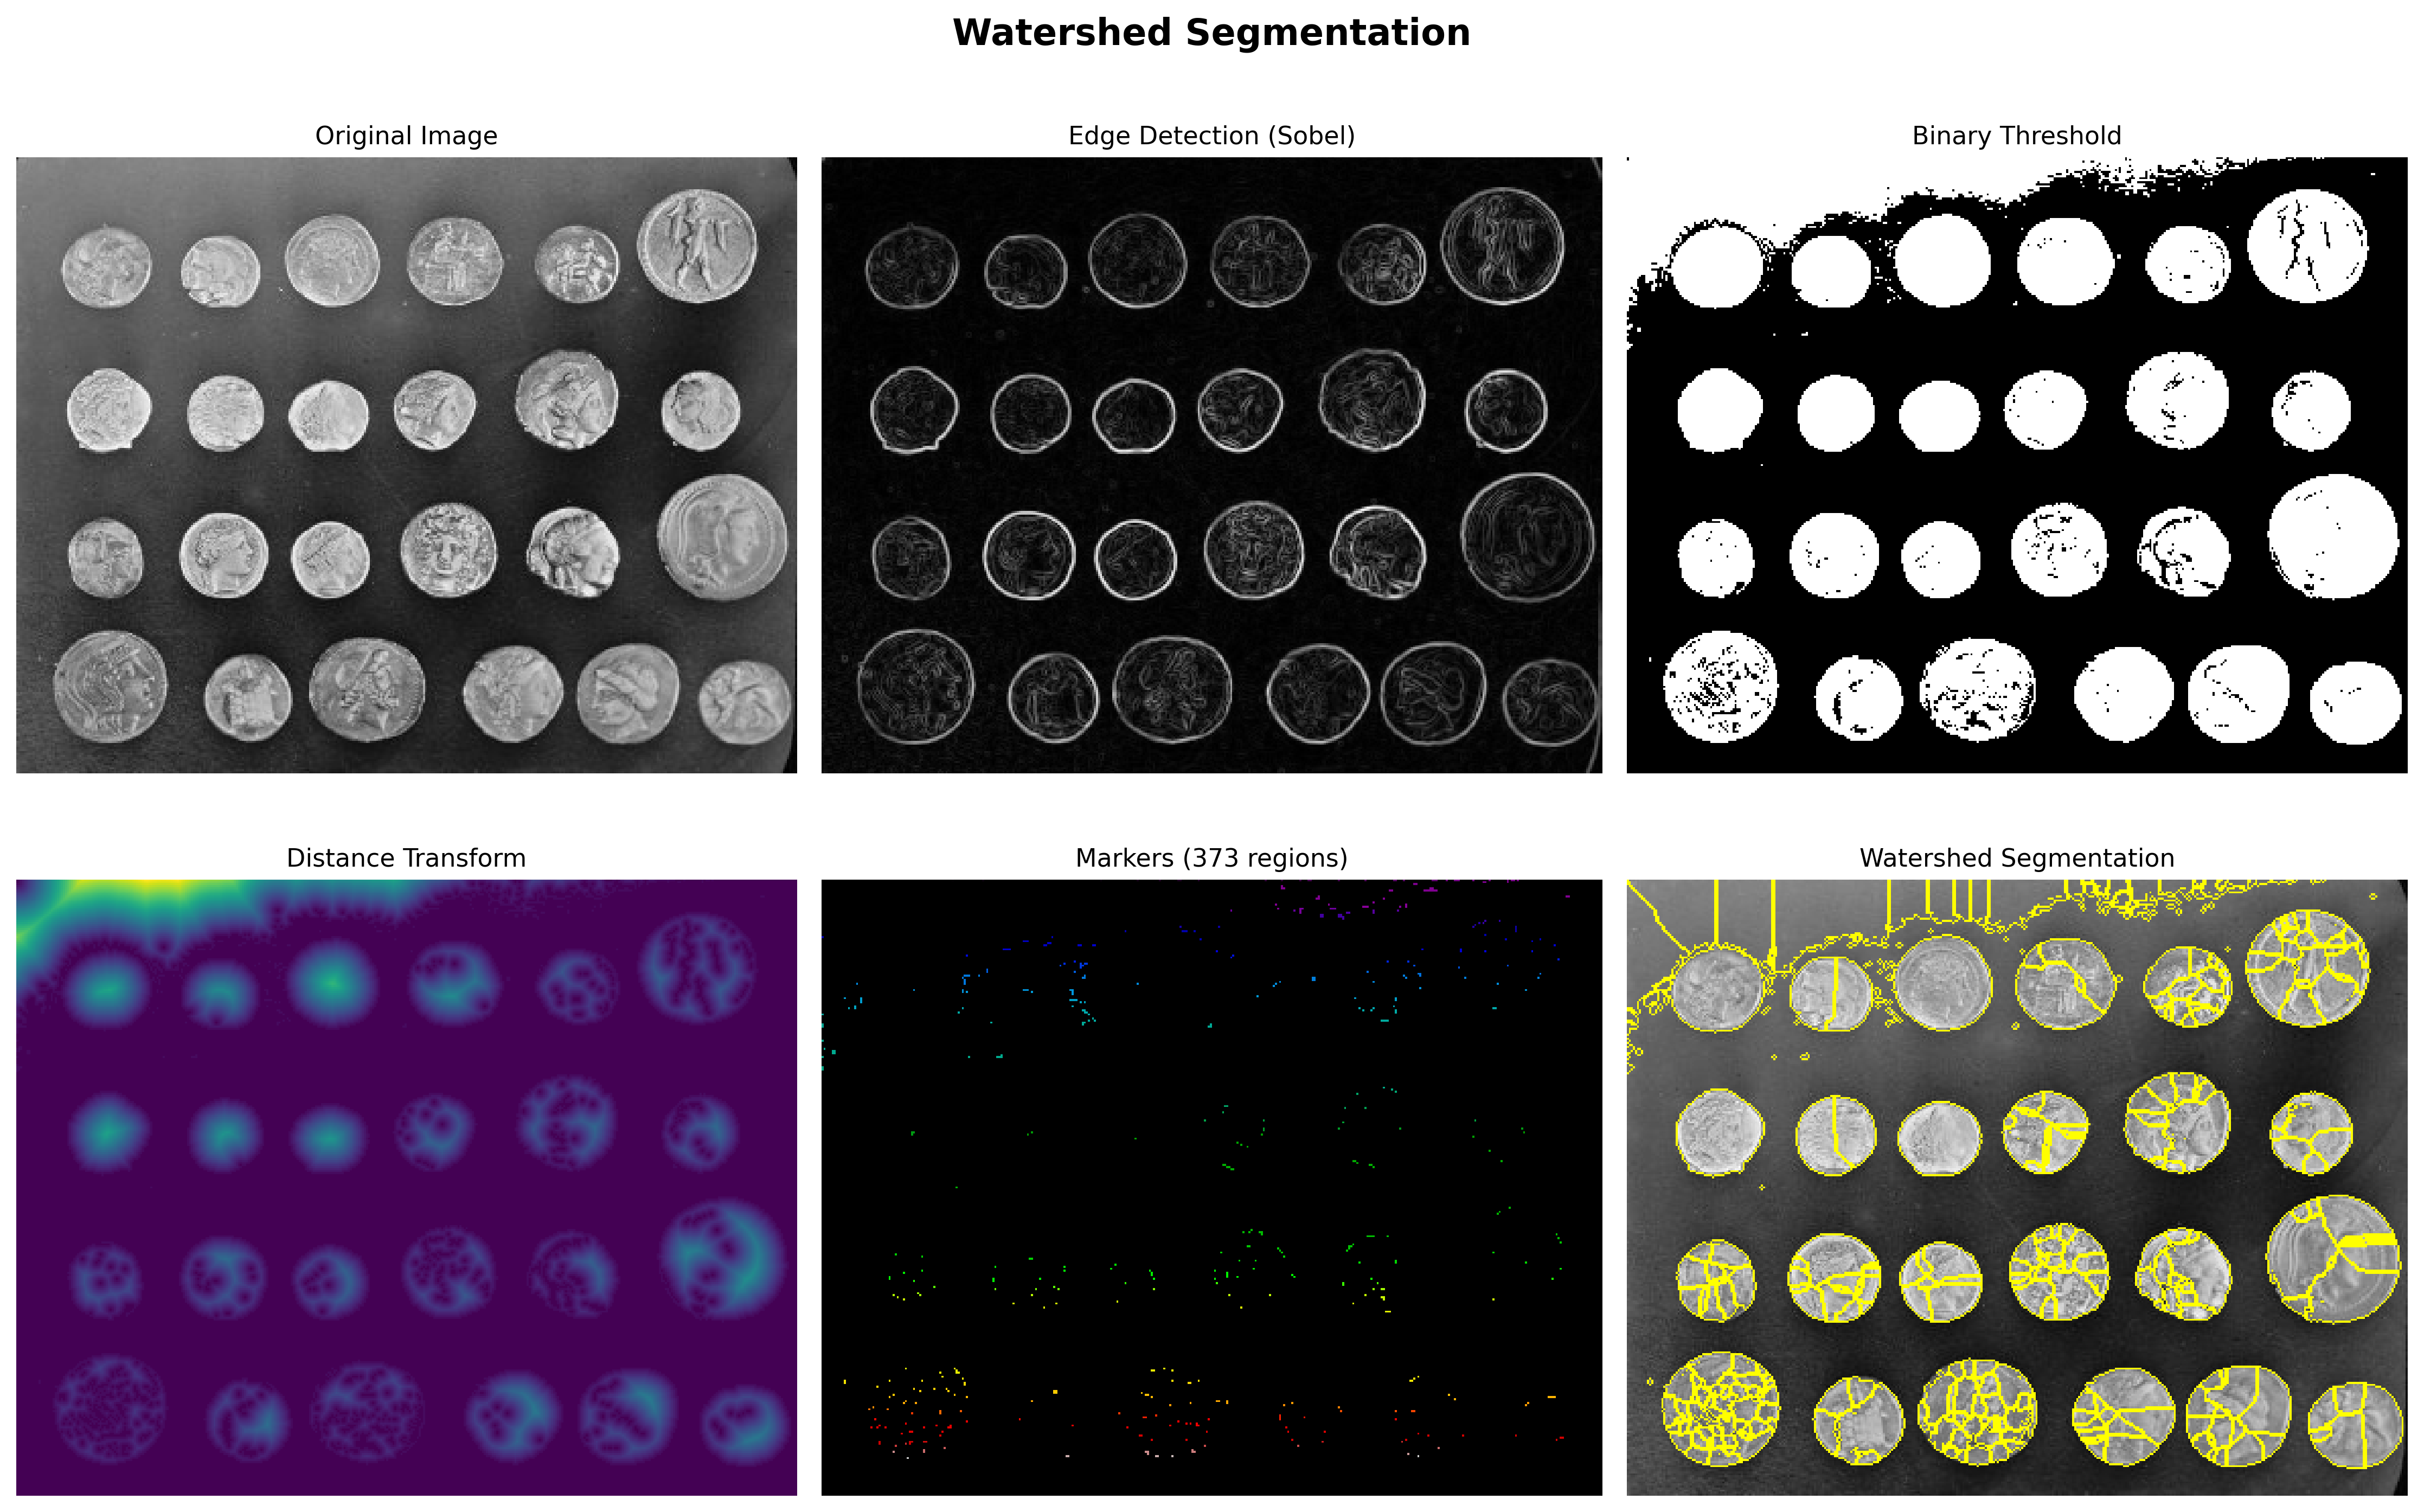
\includegraphics[width=0.92\textwidth,height=0.75\textheight,keepaspectratio]{../figures/05_watershed_segmentation.png}
\end{center}
\end{frame}

\section{Mathematical Morphology}

\begin{frame}{Introduction to Morphology}
\begin{alertblock}{Definition}
Mathematical morphology is a theory for the analysis of spatial structures based on set theory, lattice theory, and topology.
\end{alertblock}

\textbf{Foundation:} Operations based on shape (structuring element)

\textbf{Applications:}
\begin{itemize}
\item Noise removal
\item Shape analysis
\item Edge detection
\item Texture analysis
\item Object extraction
\end{itemize}
\end{frame}

\begin{frame}{Structuring Element (SE)}
\textbf{Definition:} Small shape (kernel) used to probe and modify images

\textbf{Common shapes:}
\begin{itemize}
\item Disk: Isotropic operations
\item Square/Rectangle: Directional processing
\item Diamond: 4-connected neighborhoods
\item Cross: Specific directional emphasis
\end{itemize}

\textbf{Mathematical notation:}
Let $B$ be a structuring element with origin at point $b$

The SE is translated over the image to perform morphological operations
\end{frame}

\section{Binary Morphology}

\begin{frame}{Erosion}
\textbf{Definition:} Shrinks or thins objects by removing boundary pixels

\textbf{Mathematical formulation:}
$$A \ominus B = \{z \in E \mid B_z \subseteq A\}$$

where $B_z$ is SE $B$ translated to point $z$

\textbf{Interpretation:}
\begin{itemize}
\item Output pixel is 1 if SE fits entirely inside foreground
\item Removes small protrusions
\item Separates touching objects
\item Reduces object size
\end{itemize}
\end{frame}

\begin{frame}{Dilation}
\textbf{Definition:} Expands or thickens objects by adding pixels to boundaries

\textbf{Mathematical formulation:}
$$A \oplus B = \{z \in E \mid (\hat{B})_z \cap A \neq \emptyset\}$$

where $\hat{B}$ is the reflection of $B$

\textbf{Interpretation:}
\begin{itemize}
\item Output pixel is 1 if SE overlaps with foreground
\item Fills small holes
\item Connects nearby objects
\item Increases object size
\end{itemize}
\end{frame}

\begin{frame}{Erosion and Dilation: Visual Results}
\begin{center}
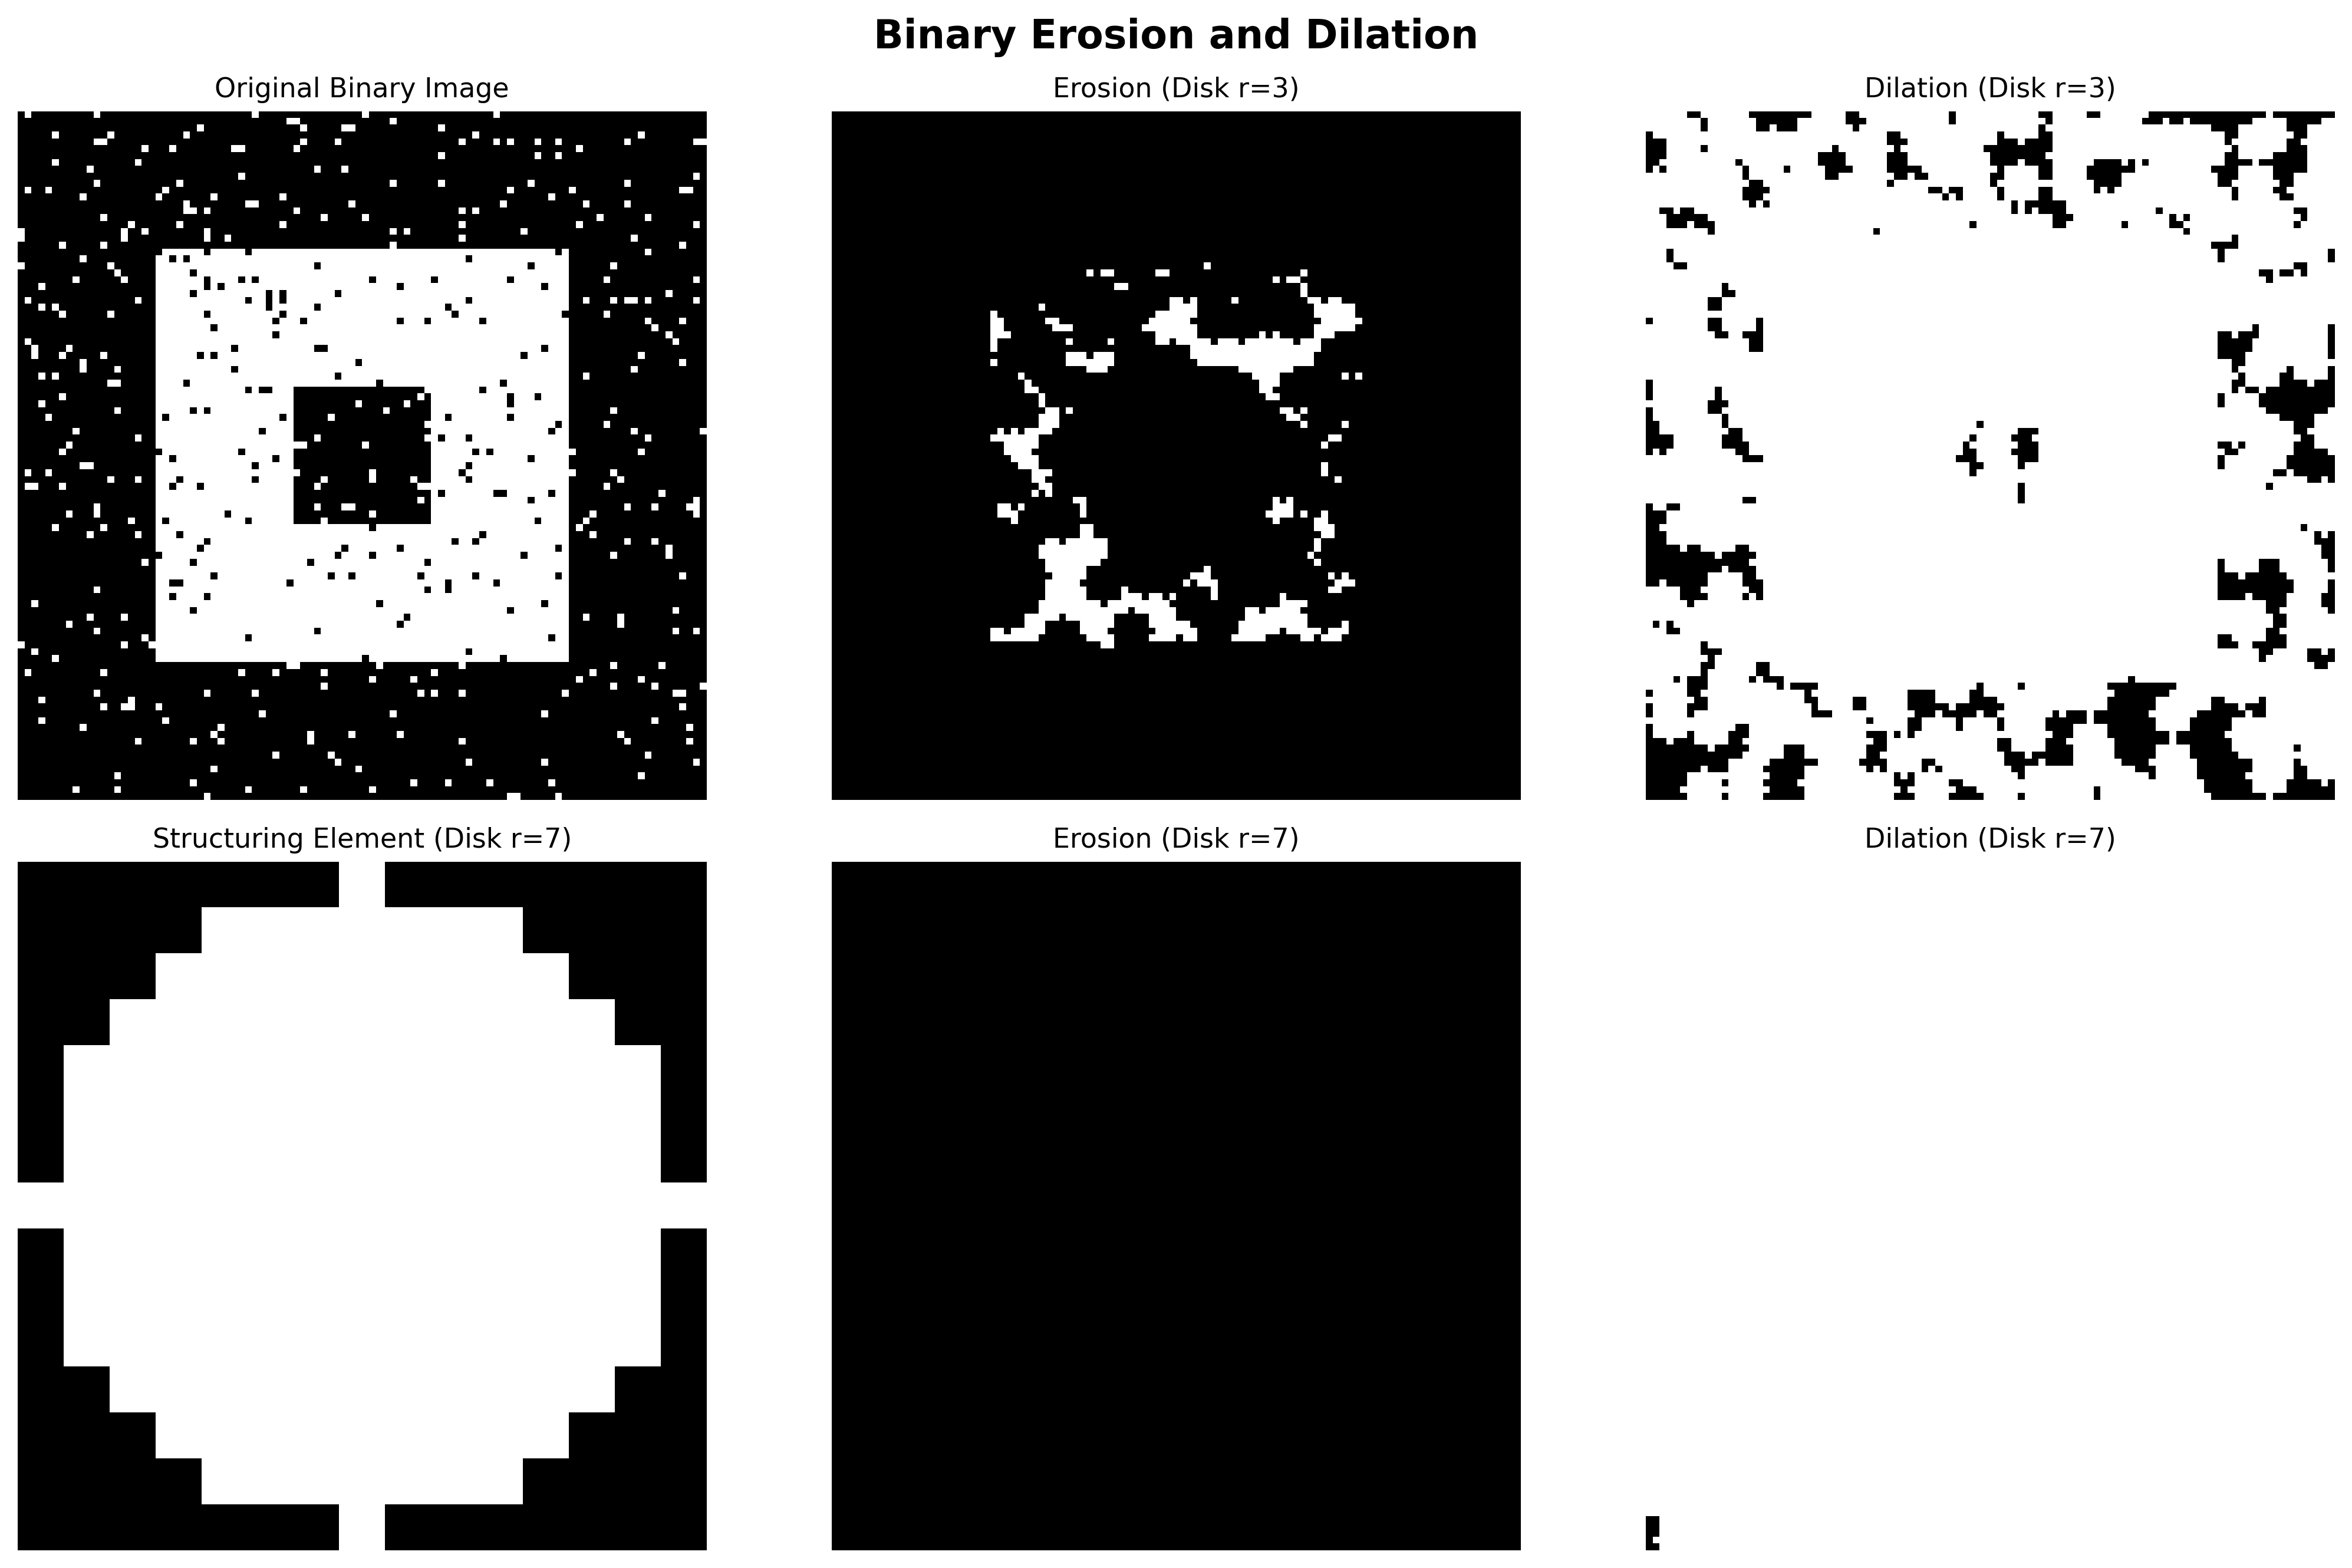
\includegraphics[width=0.92\textwidth,height=0.73\textheight,keepaspectratio]{../figures/06_binary_erosion_dilation.png}
\end{center}
\end{frame}

\begin{frame}{Duality of Erosion and Dilation}
\textbf{Fundamental relationship:}
$$(A \ominus B)^c = A^c \oplus \hat{B}$$
$$(A \oplus B)^c = A^c \ominus \hat{B}$$

where $A^c$ denotes complement and $\hat{B}$ is reflection

\textbf{Practical implication:}
Eroding the foreground = dilating the background

This duality enables efficient implementation and theoretical analysis
\end{frame}

\begin{frame}{Opening}
\textbf{Definition:} Erosion followed by dilation

$$A \circ B = (A \ominus B) \oplus B$$

\textbf{Properties:}
\begin{itemize}
\item Removes small bright regions (noise)
\item Smooths object contours
\item Breaks narrow connections
\item Preserves object size (approximately)
\item Idempotent: $(A \circ B) \circ B = A \circ B$
\end{itemize}

\textbf{Use case:} Noise removal while preserving object shape
\end{frame}

\begin{frame}{Closing}
\textbf{Definition:} Dilation followed by erosion

$$A \bullet B = (A \oplus B) \ominus B$$

\textbf{Properties:}
\begin{itemize}
\item Fills small dark regions (holes)
\item Smooths object contours
\item Fuses narrow gaps
\item Preserves object size (approximately)
\item Idempotent: $(A \bullet B) \bullet B = A \bullet B$
\end{itemize}

\textbf{Use case:} Fill holes and gaps in objects
\end{frame}

\begin{frame}{Opening and Closing: Results}
\begin{center}
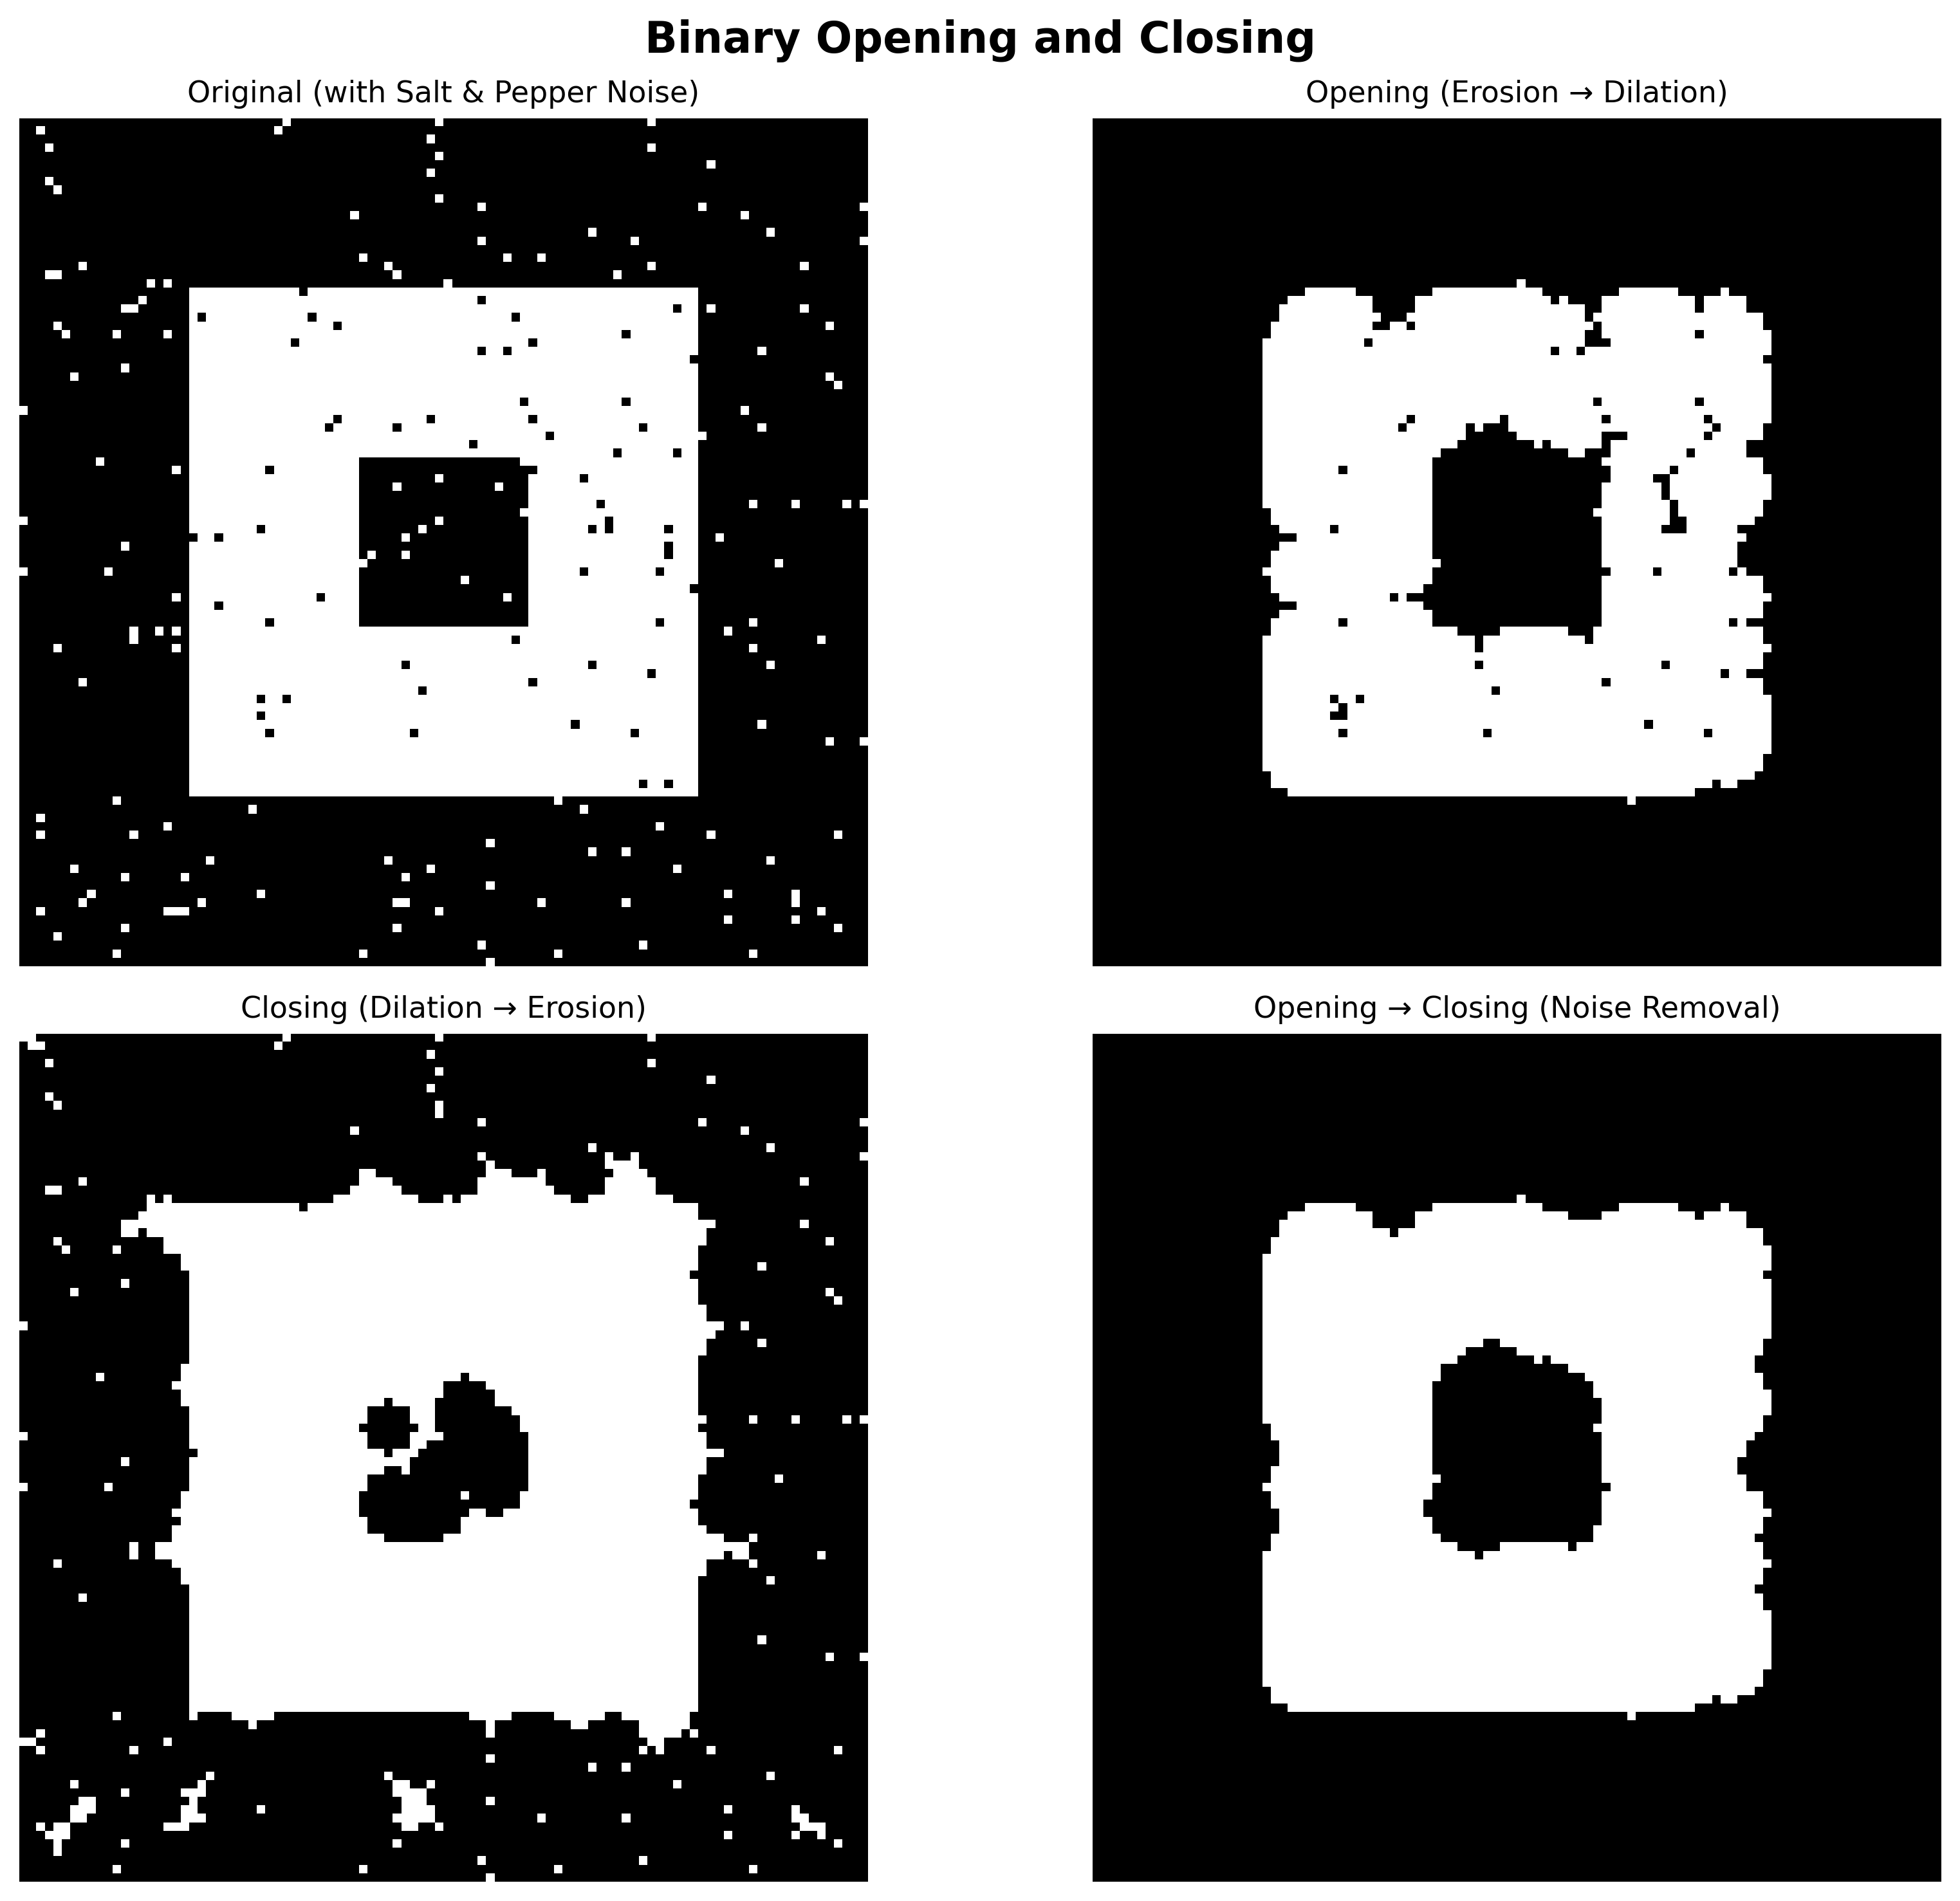
\includegraphics[width=0.8\textwidth,height=0.63\textheight,keepaspectratio]{../figures/07_binary_opening_closing.png}
\end{center}
\end{frame}

\begin{frame}{Morphological Properties}
\textbf{Translation invariance:}
$$(A + h) \ominus B = (A \ominus B) + h$$

\textbf{Increasing:}
$$A_1 \subseteq A_2 \Rightarrow A_1 \ominus B \subseteq A_2 \ominus B$$

\textbf{Distributivity over intersection:}
$$(A \cap B) \ominus C = (A \ominus C) \cap (B \ominus C)$$

\textbf{Opening and closing relationship:}
$$A \circ B \subseteq A \subseteq A \bullet B$$
\end{frame}

\begin{frame}{Structuring Element Design}
\begin{center}
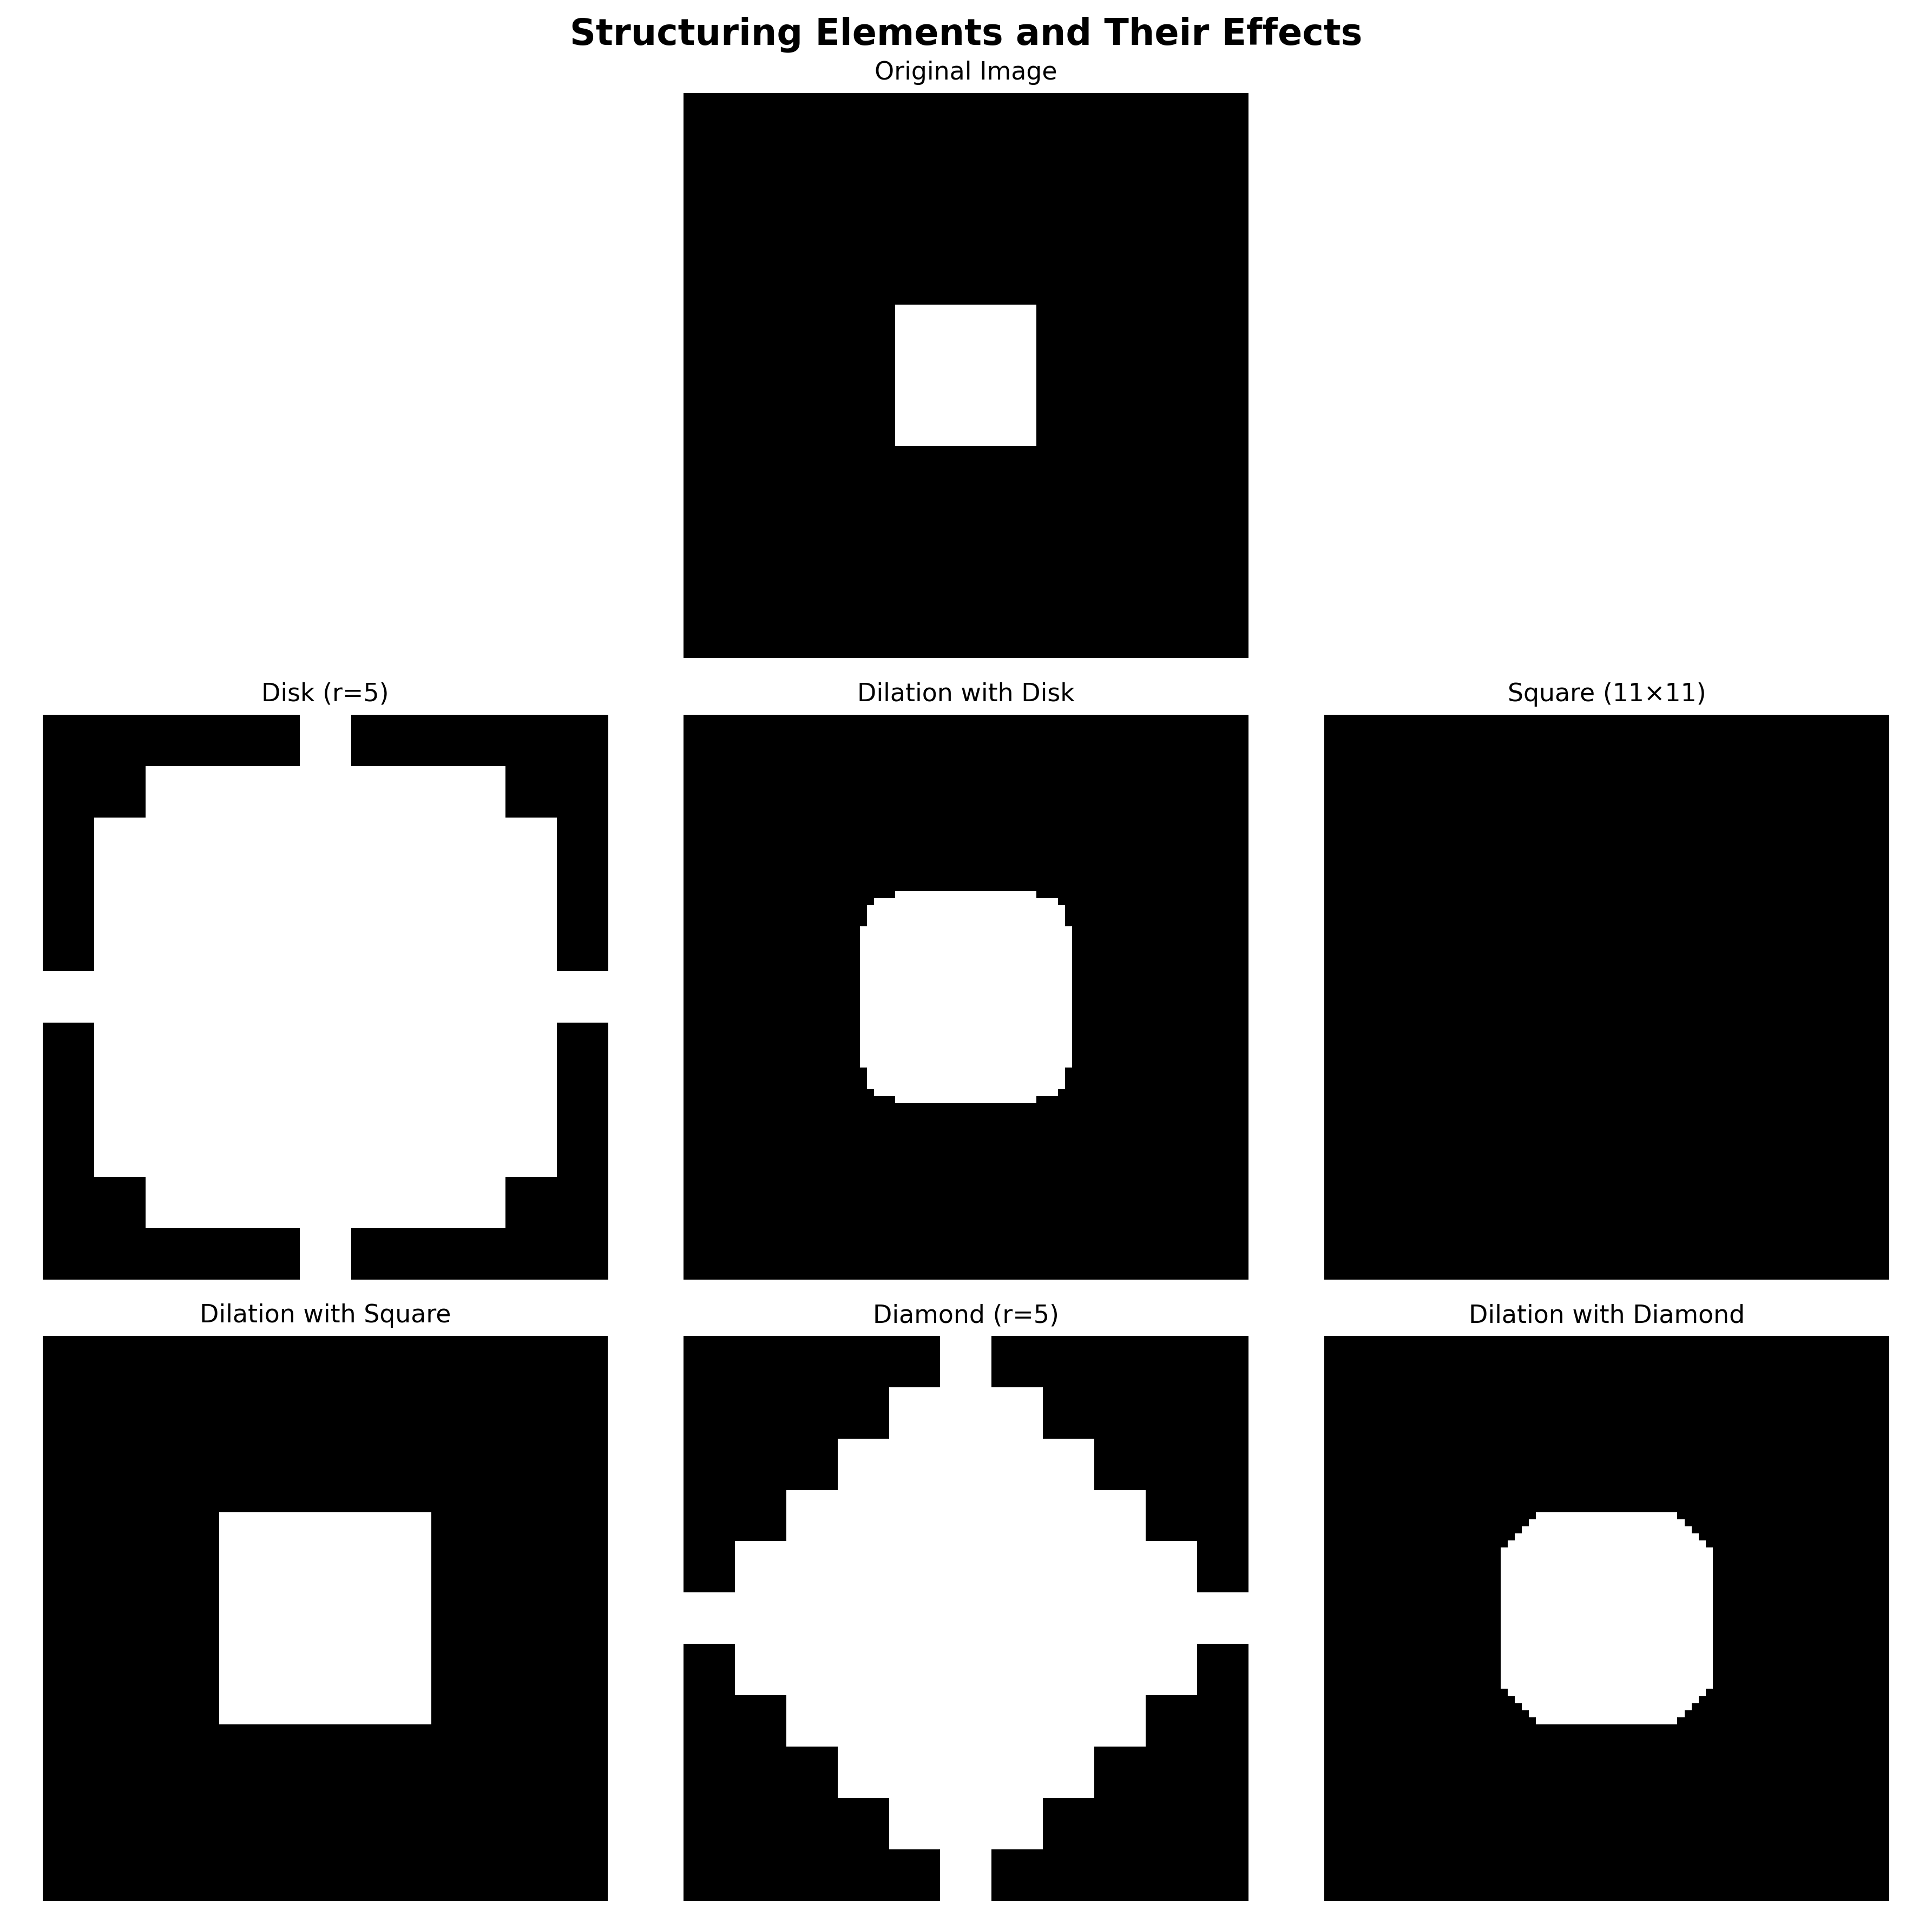
\includegraphics[width=0.78\textwidth,height=0.6\textheight,keepaspectratio]{../figures/08_structuring_elements.png}
\end{center}
\end{frame}

\section{Grayscale Morphology}

\begin{frame}{Grayscale Erosion and Dilation}
\textbf{Grayscale erosion:}
$$(f \ominus b)(x,y) = \min_{(s,t) \in b} \{f(x+s, y+t) - b(s,t)\}$$

\textbf{Grayscale dilation:}
$$(f \oplus b)(x,y) = \max_{(s,t) \in b} \{f(x+s, y+t) + b(s,t)\}$$

\textbf{Flat structuring element ($b(s,t) = 0$):}
\begin{itemize}
\item Erosion: Local minimum filter
\item Dilation: Local maximum filter
\end{itemize}
\end{frame}

\begin{frame}{Grayscale Opening and Closing}
\textbf{Opening:}
$$f \circ b = (f \ominus b) \oplus b$$
\begin{itemize}
\item Removes bright details smaller than SE
\item Darkens the image
\end{itemize}

\textbf{Closing:}
$$f \bullet b = (f \oplus b) \ominus b$$
\begin{itemize}
\item Removes dark details smaller than SE
\item Brightens the image
\end{itemize}
\end{frame}

\begin{frame}{Morphological Gradient}
\textbf{Gradient:}
$$(f \oplus b) - (f \ominus b)$$
Highlights edges and boundaries

\textbf{Internal gradient:}
$$f - (f \ominus b)$$
Emphasizes internal edges

\textbf{External gradient:}
$$(f \oplus b) - f$$
Emphasizes external edges
\end{frame}

\begin{frame}{Morphological Gradient: Visualization}
\begin{center}
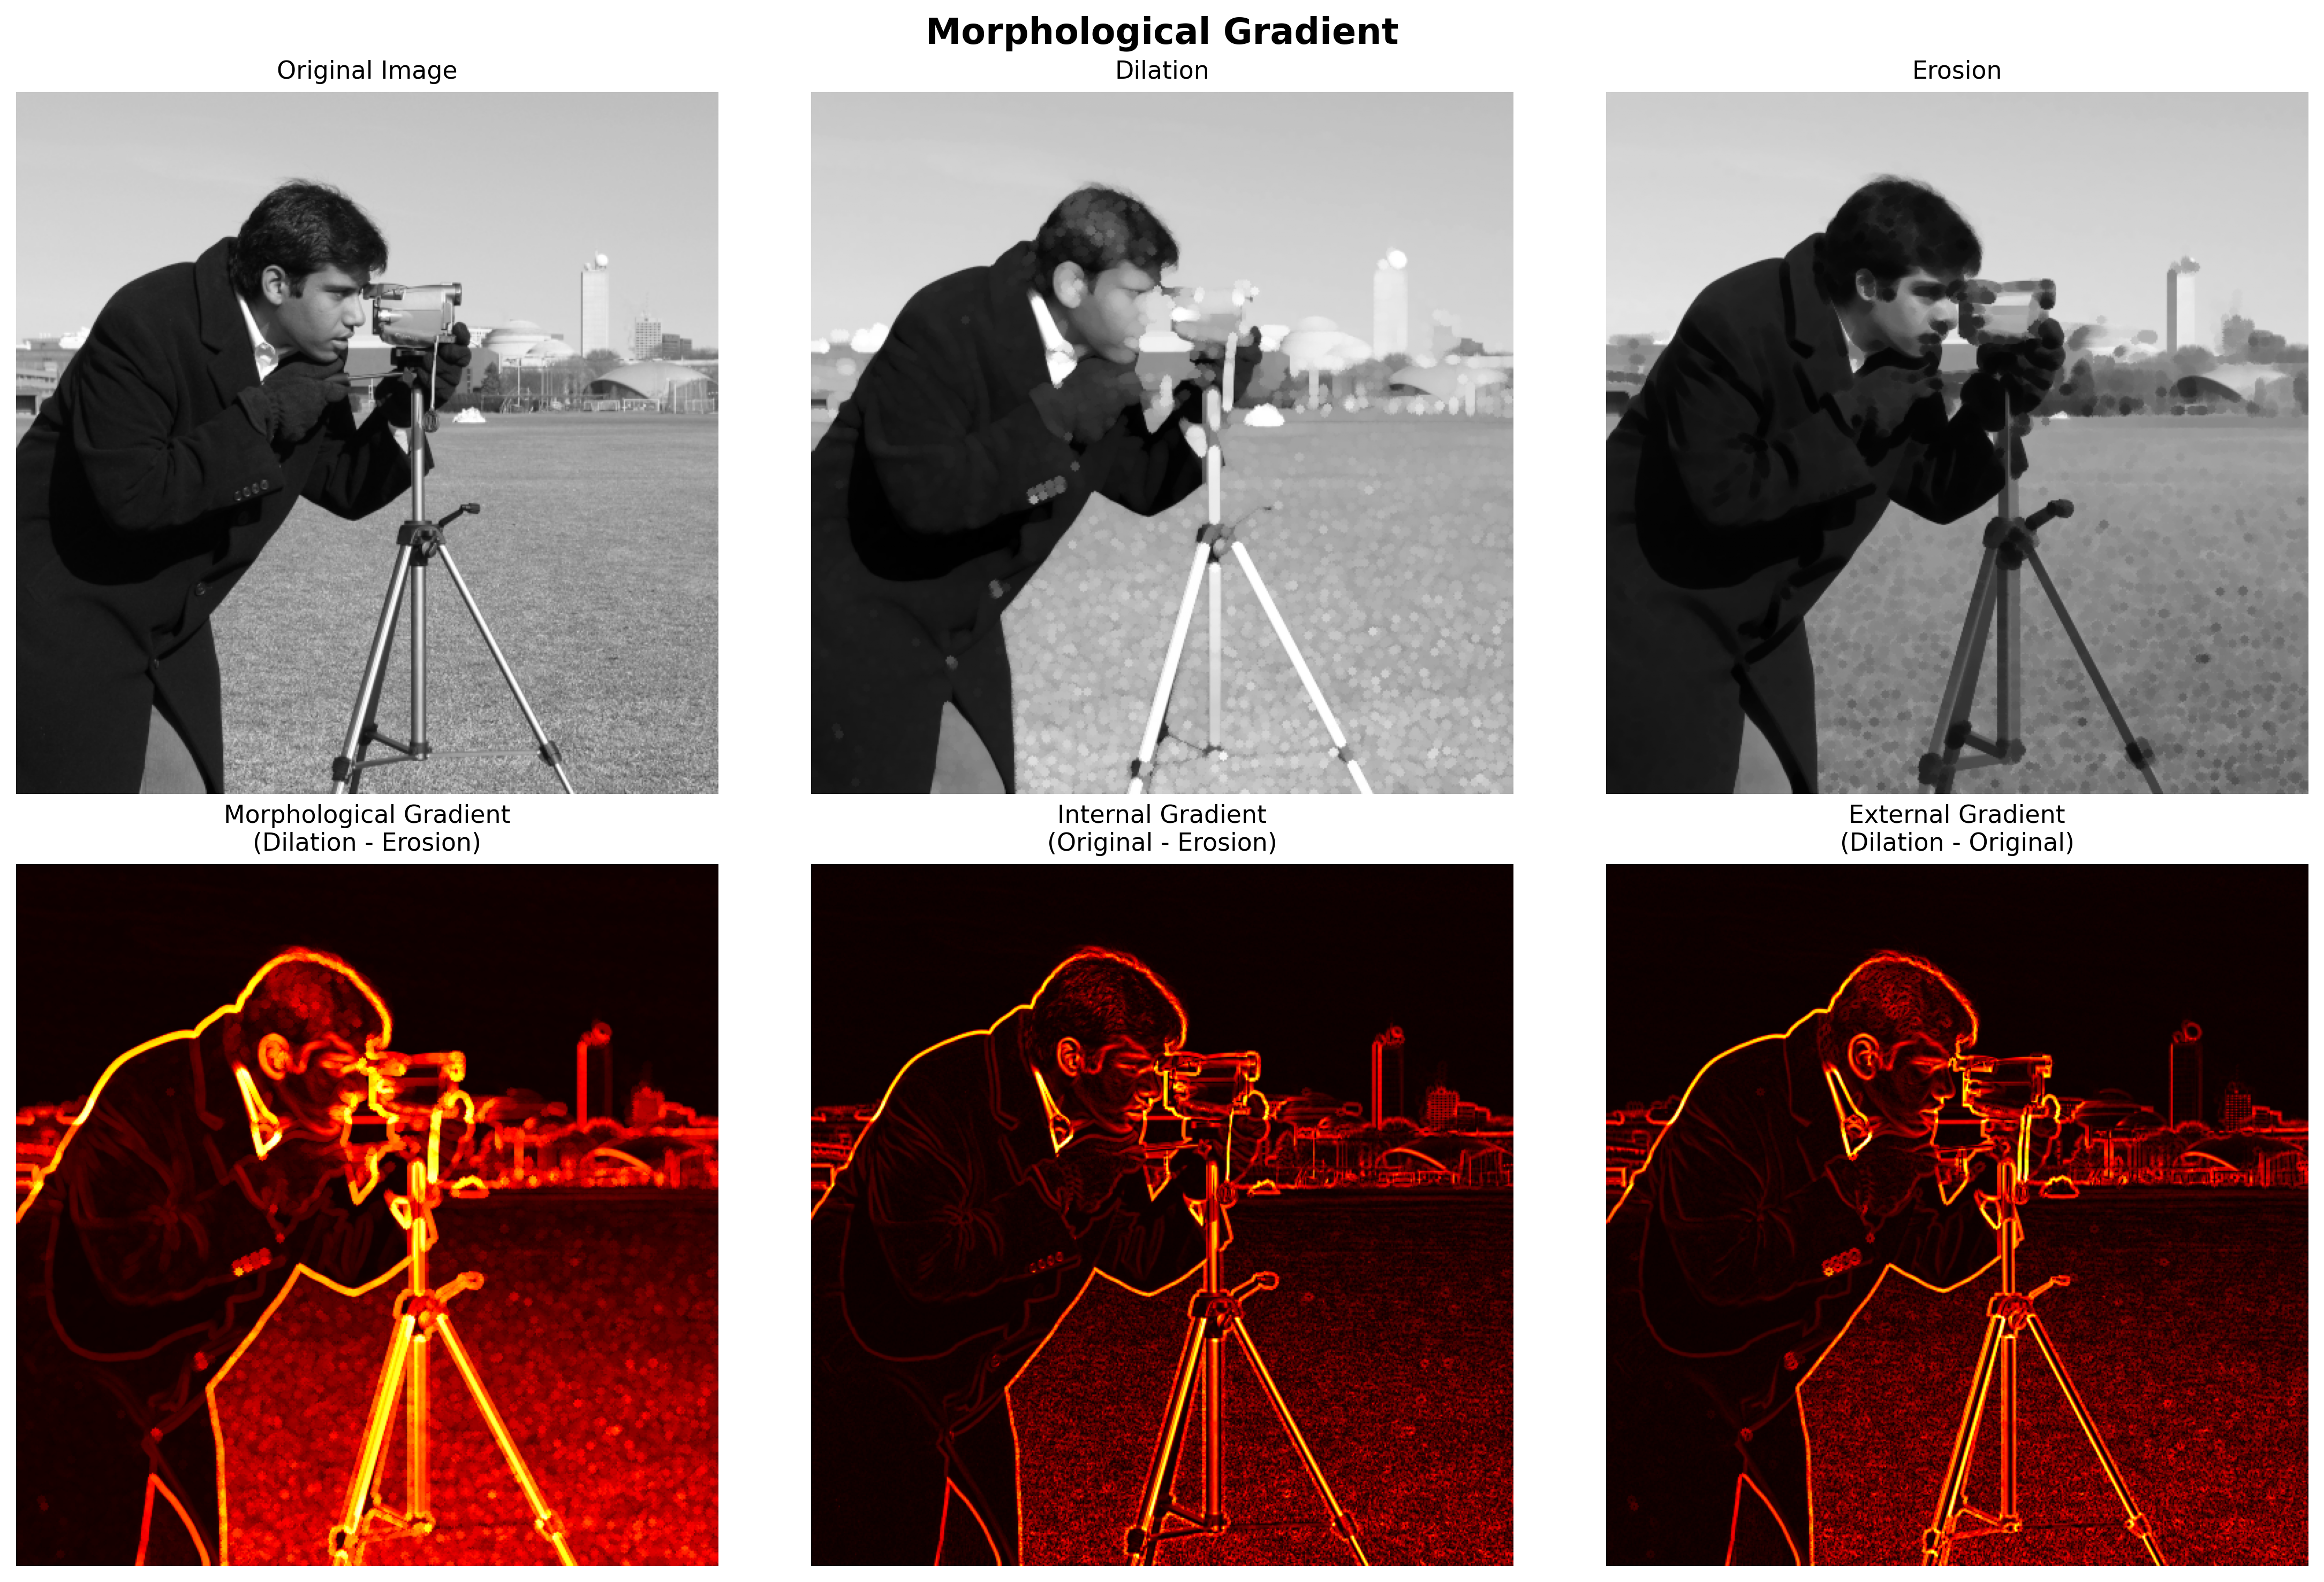
\includegraphics[width=0.92\textwidth,height=0.73\textheight,keepaspectratio]{../figures/09_morphological_gradient.png}
\end{center}
\end{frame}

\begin{frame}{Top-Hat Transforms}
\textbf{White top-hat:}
$$\text{WTH}(f) = f - (f \circ b)$$
Extracts bright features smaller than SE

\textbf{Black top-hat:}
$$\text{BTH}(f) = (f \bullet b) - f$$
Extracts dark features smaller than SE

\textbf{Applications:}
\begin{itemize}
\item Background correction
\item Feature enhancement
\item Texture analysis
\end{itemize}
\end{frame}

\begin{frame}{Grayscale Morphology: Complete Example}
\begin{center}
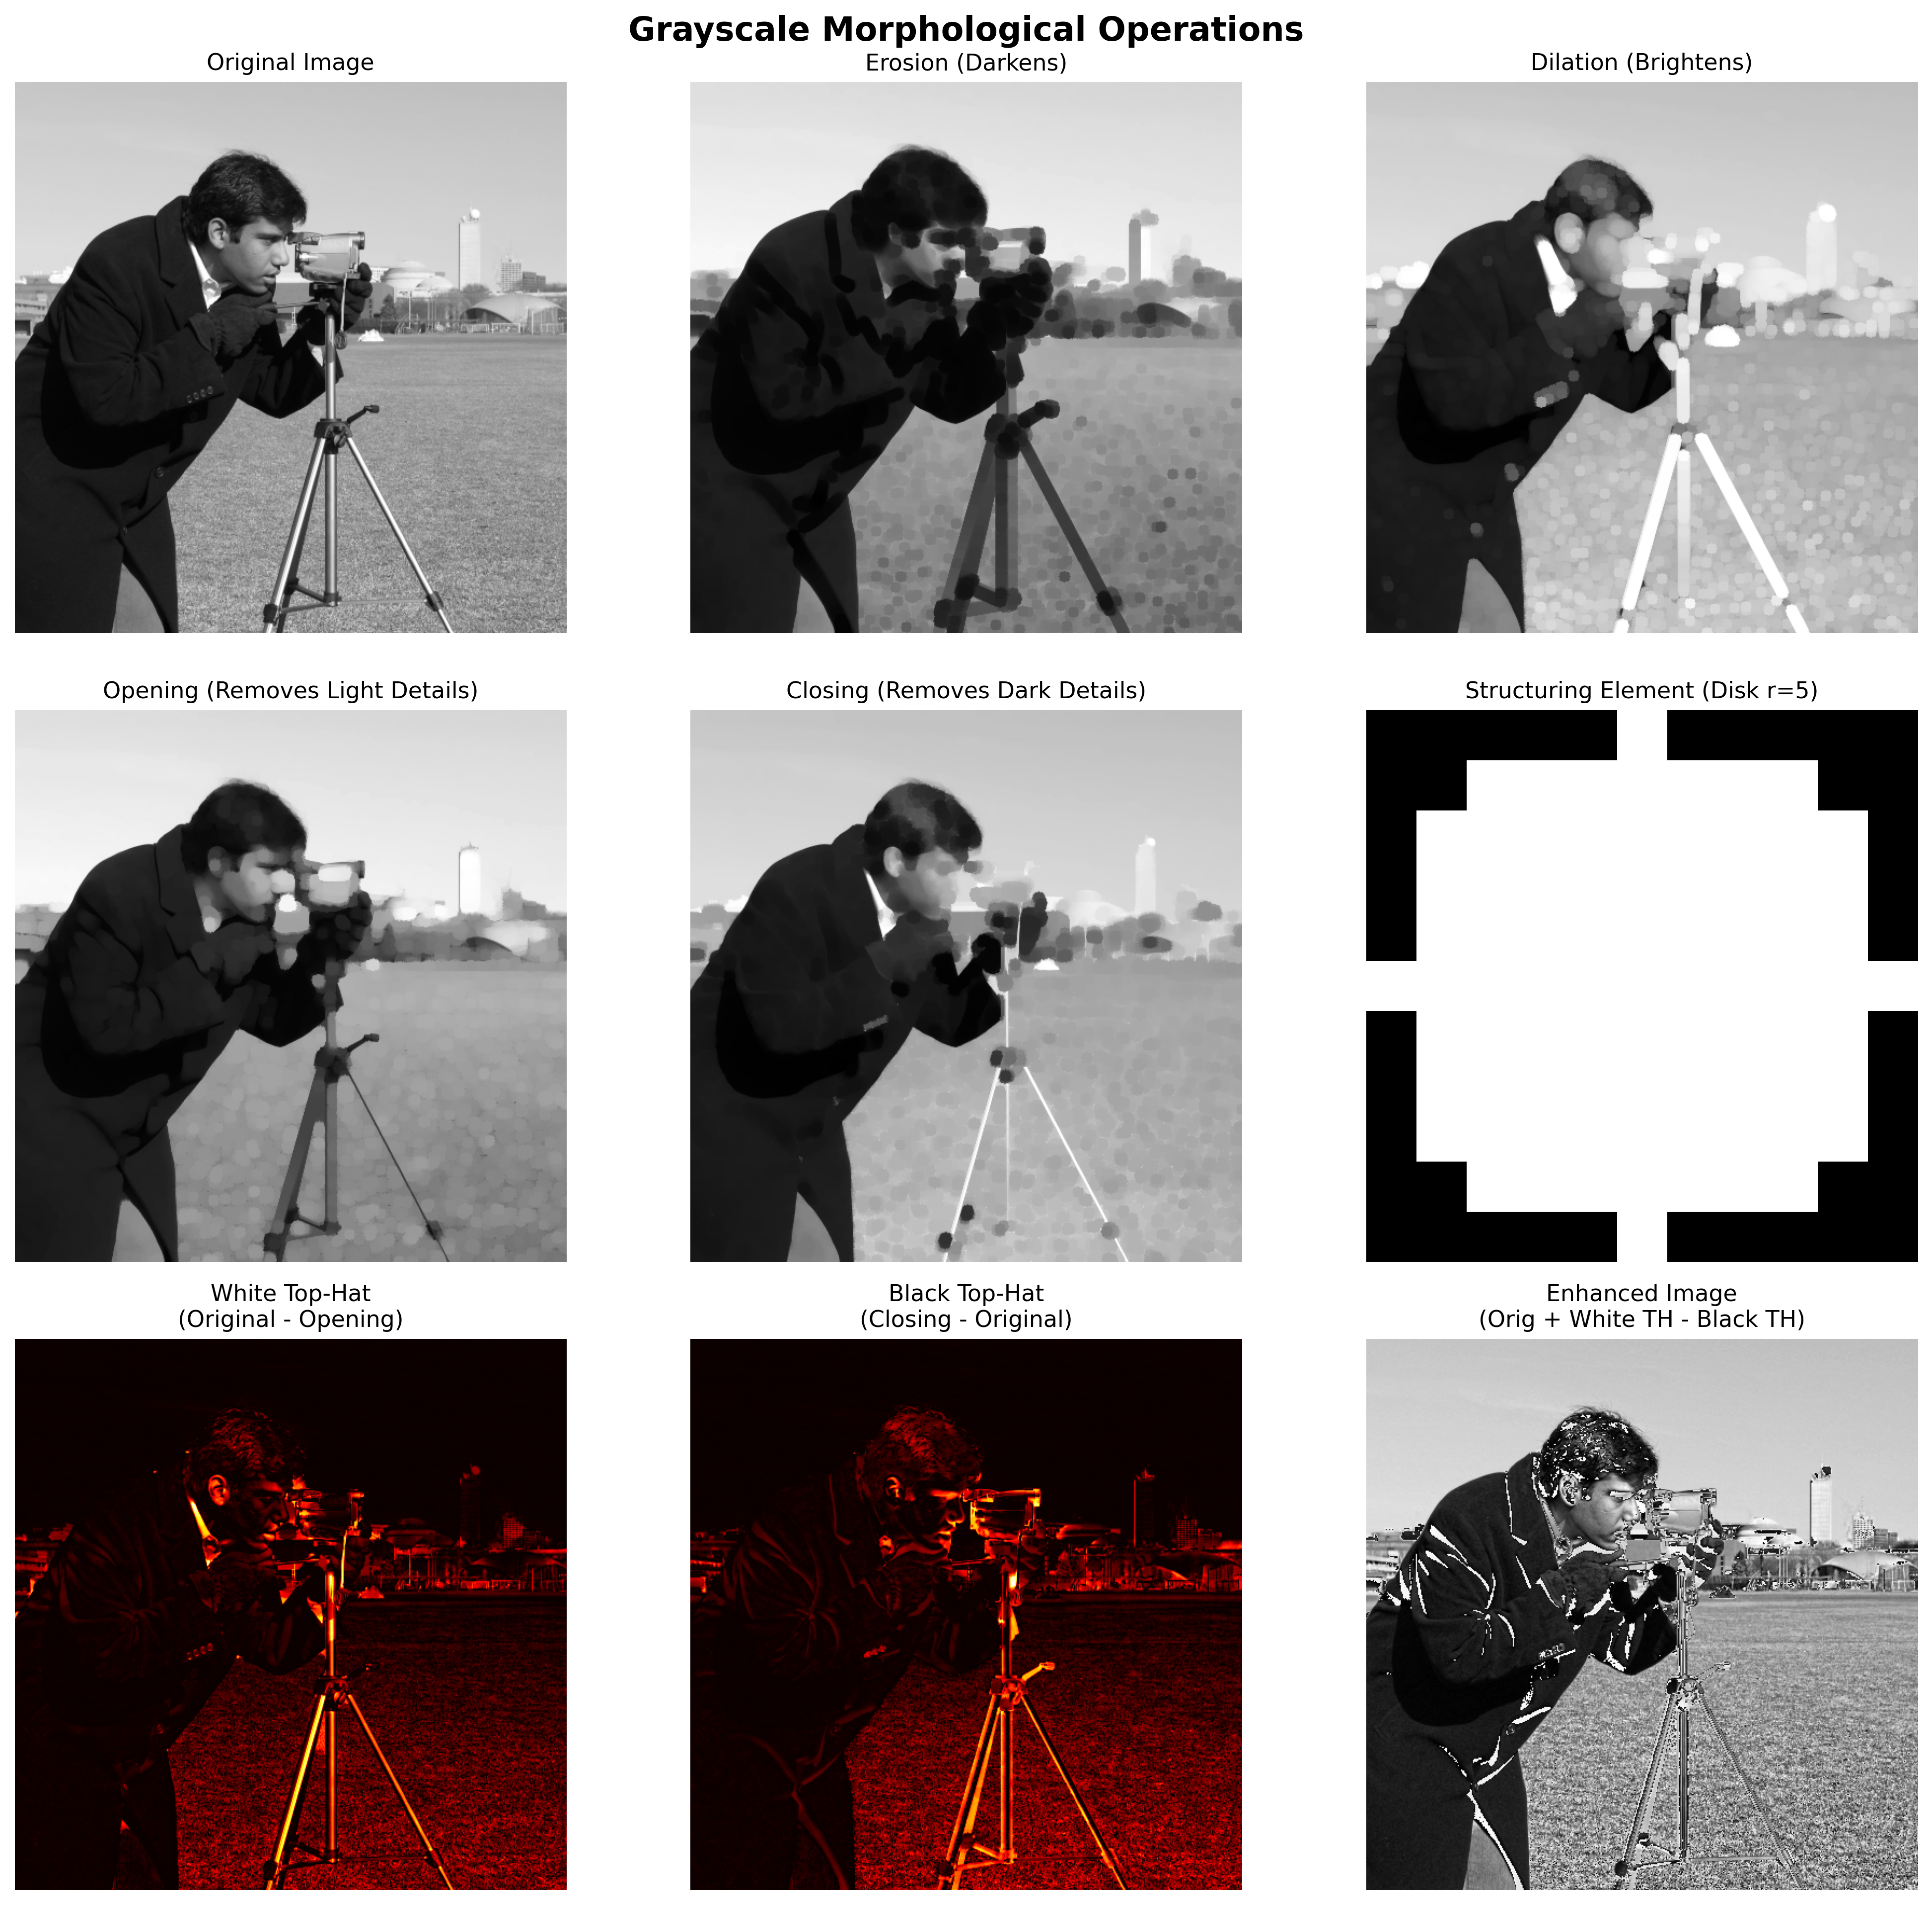
\includegraphics[width=0.82\textwidth,height=0.6\textheight,keepaspectratio]{../figures/10_grayscale_morphology.png}
\end{center}
\end{frame}

\section{Advanced Applications}

\begin{frame}{Morphological Noise Removal}
\textbf{Pipeline for binary images:}
\begin{enumerate}
\item Opening: Remove salt noise (small white regions)
\item Closing: Remove pepper noise (small black regions)
\item Remove small objects: Eliminate isolated noise
\item Fill holes: Complete object regions
\end{enumerate}

\textbf{Parameter selection:}
\begin{itemize}
\item SE size based on noise characteristics
\item Larger SE for stronger filtering
\item Trade-off: noise removal vs. detail preservation
\end{itemize}
\end{frame}

\begin{frame}{Noise Removal Pipeline: Results}
\begin{center}
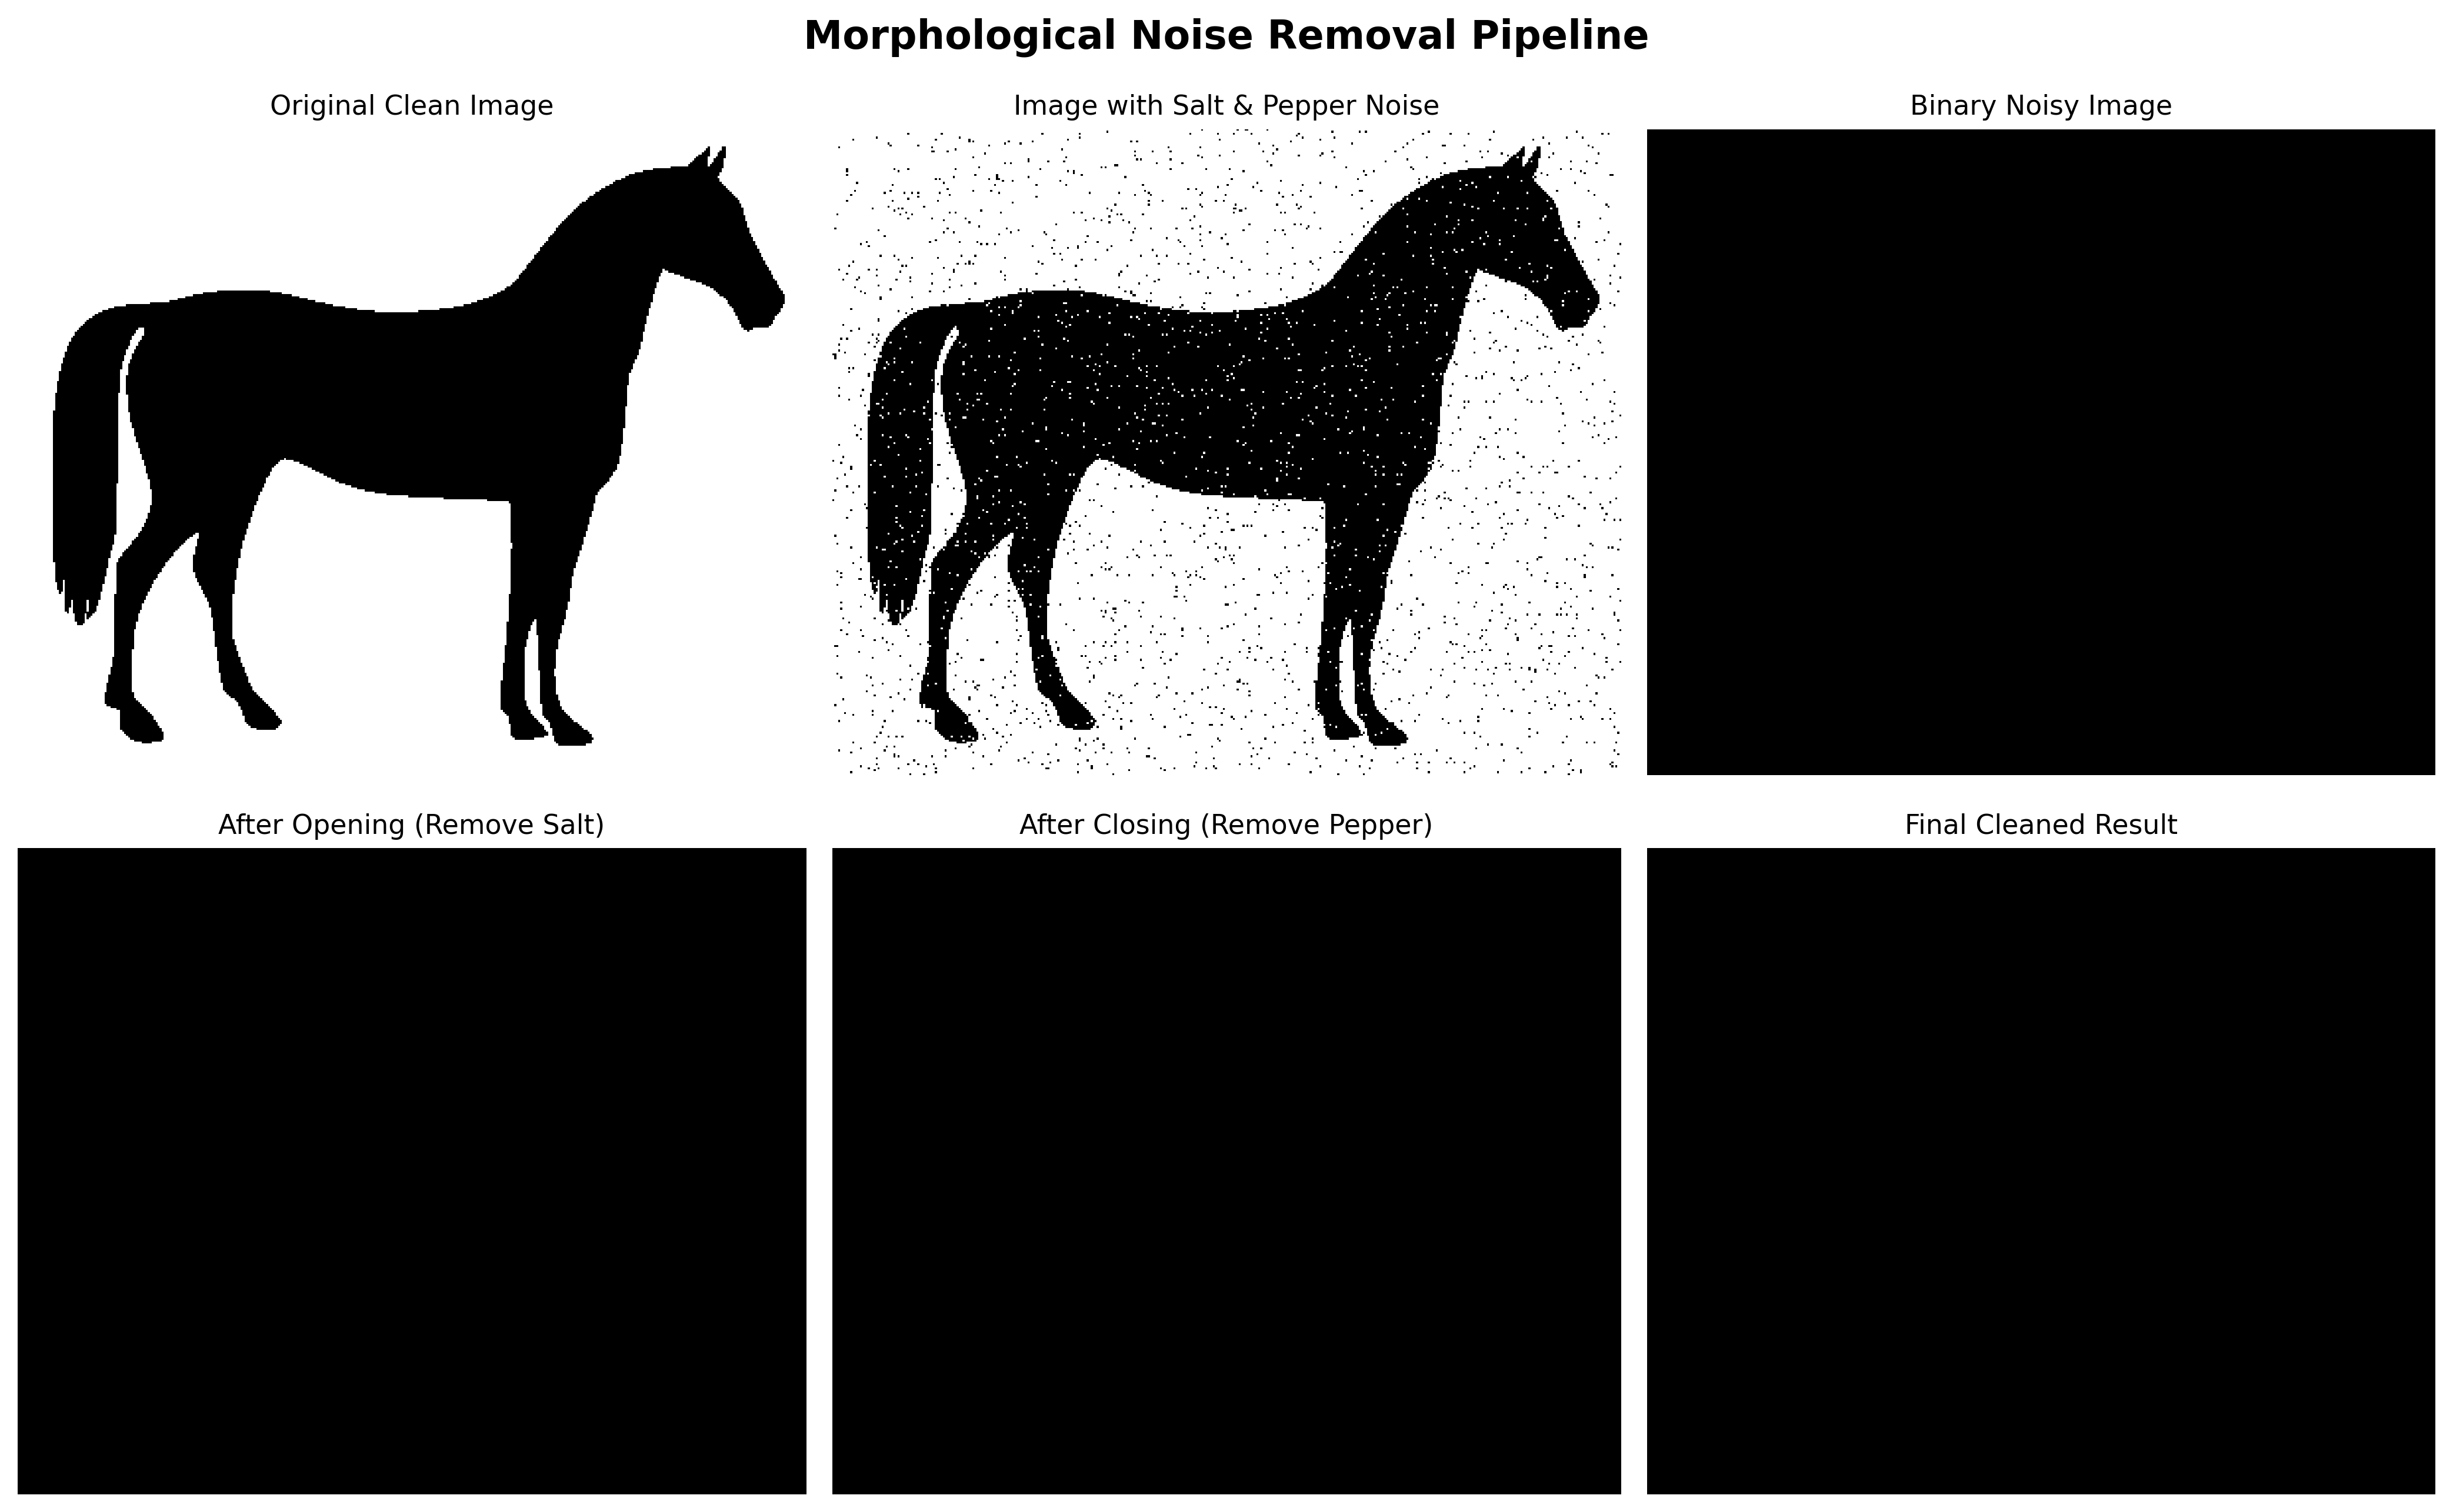
\includegraphics[width=0.92\textwidth,height=0.75\textheight,keepaspectratio]{../figures/11_noise_removal_pipeline.png}
\end{center}
\end{frame}

\begin{frame}{Edge Detection with Morphology}
\begin{center}
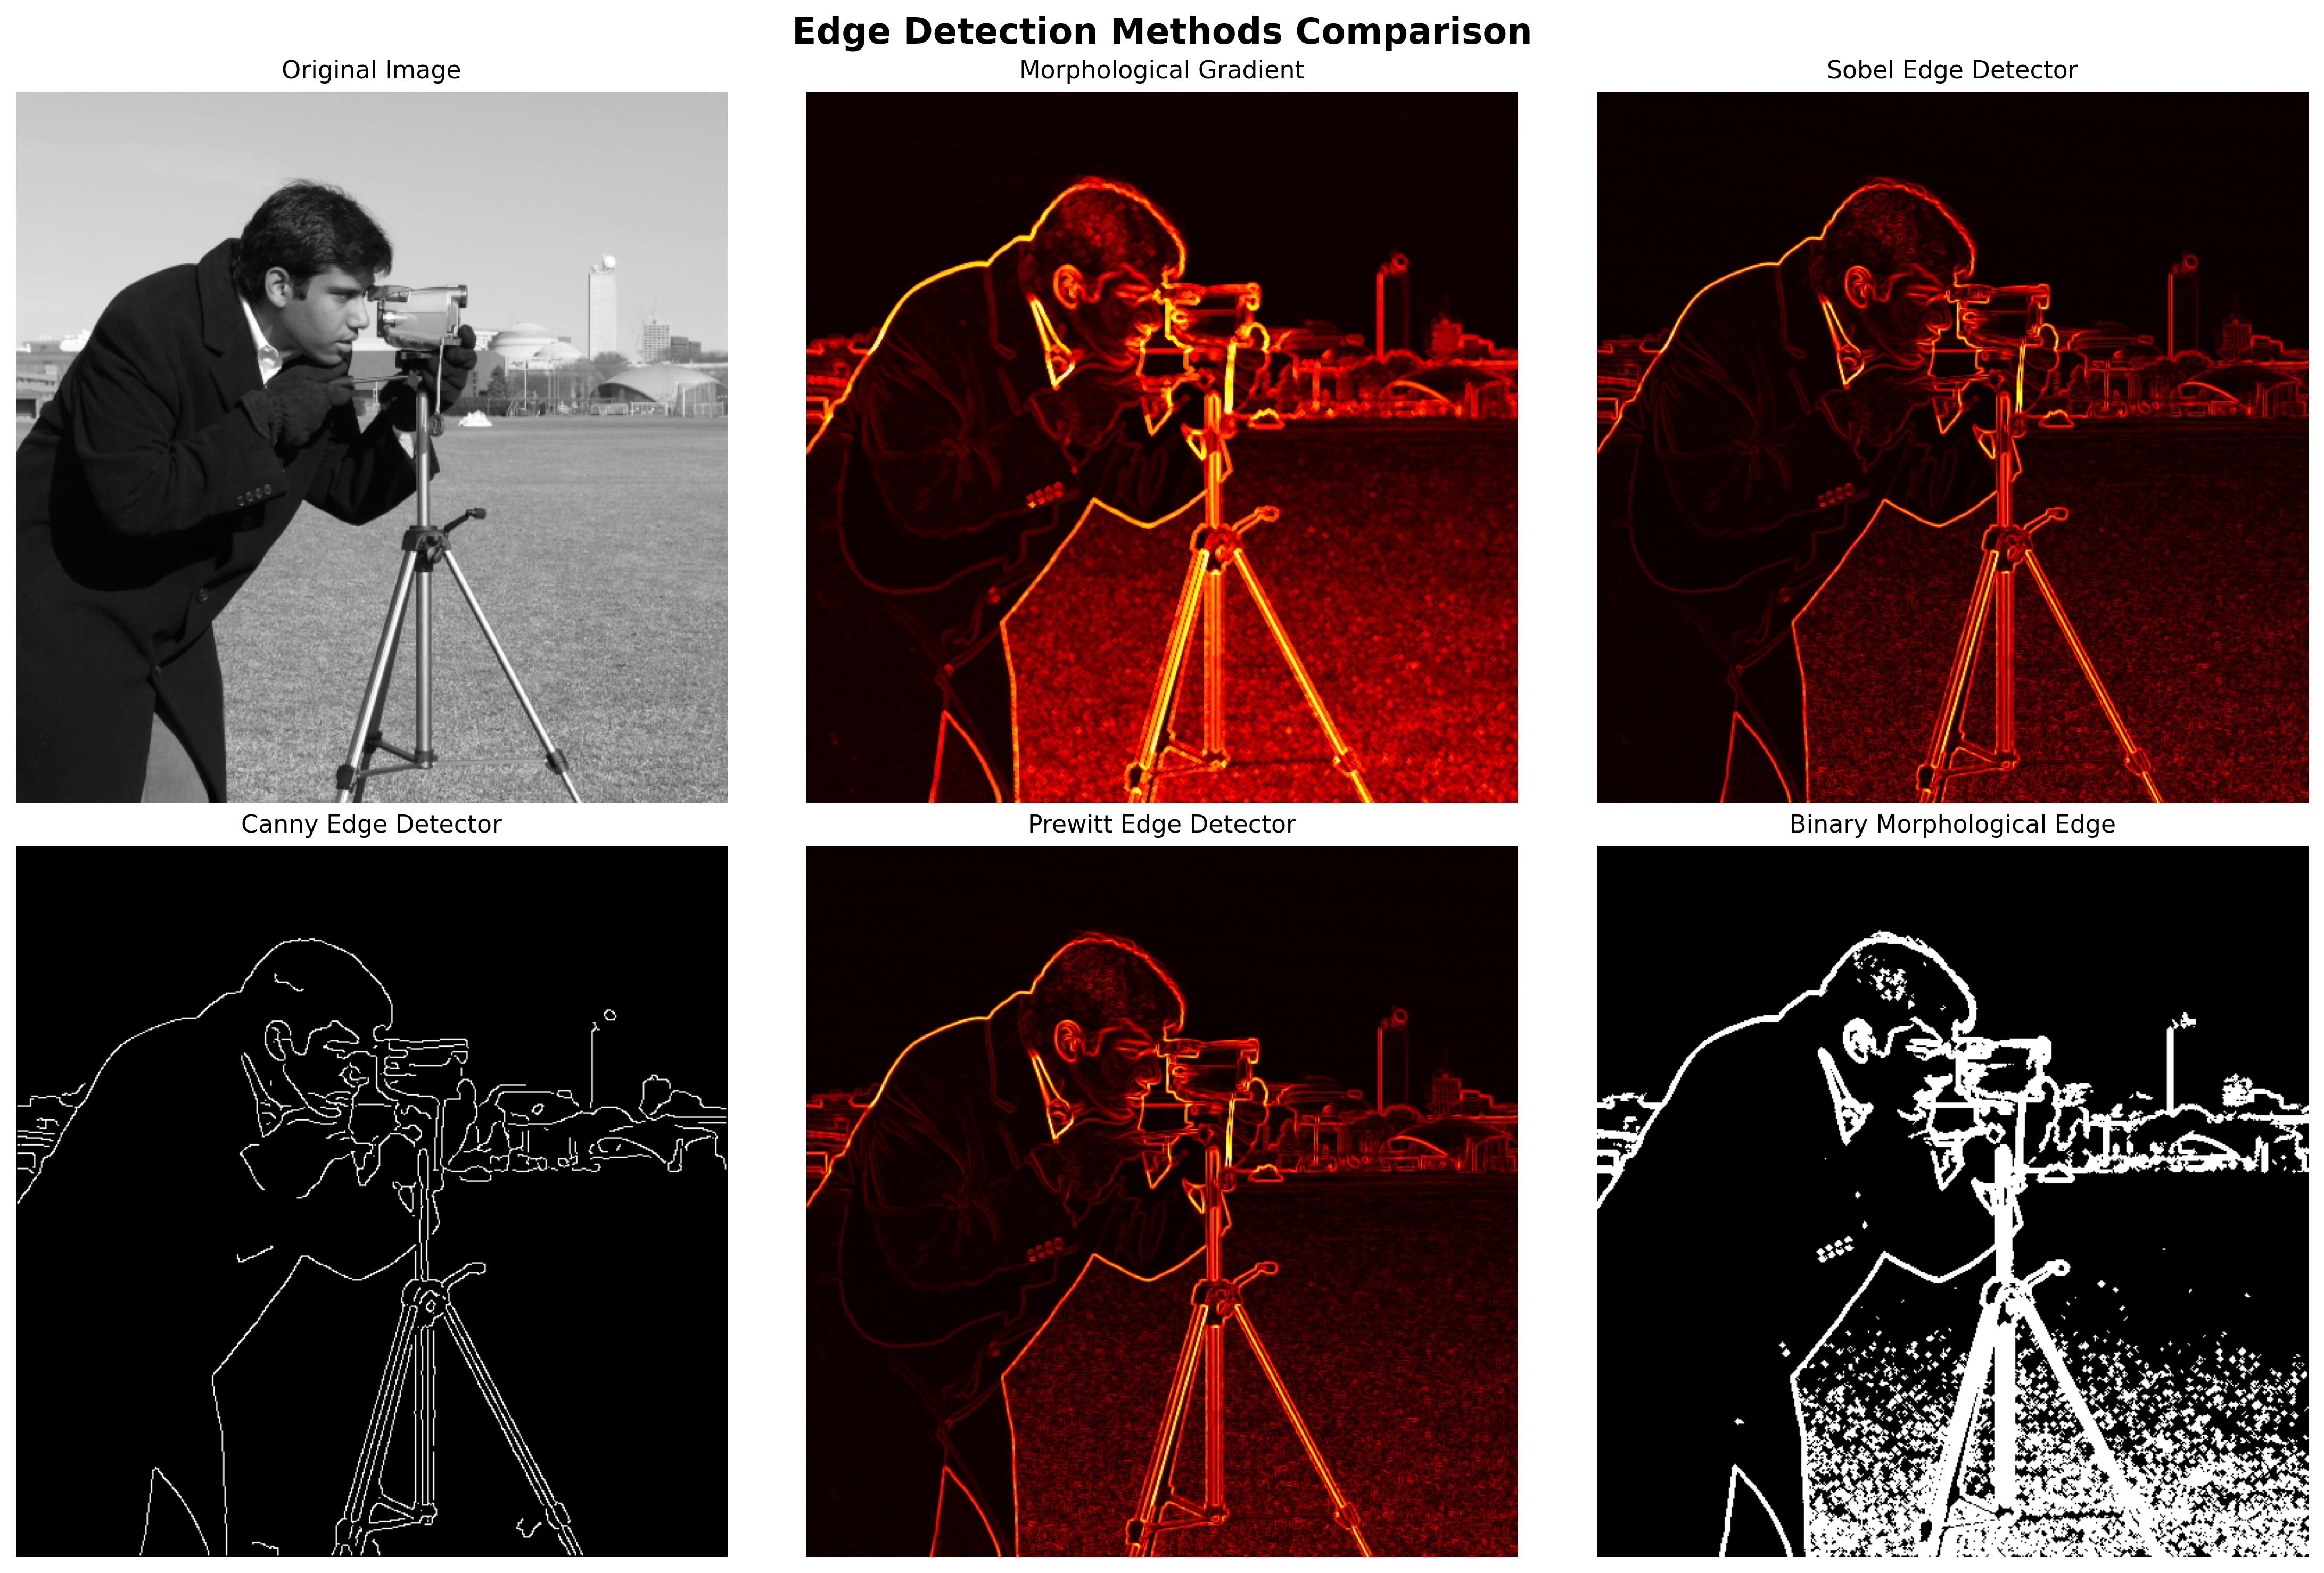
\includegraphics[width=0.9\textwidth,height=0.72\textheight,keepaspectratio]{../figures/12_edge_detection_comparison.png}
\end{center}
\end{frame}

\begin{frame}{Object Extraction and Analysis}
\textbf{Complete workflow:}
\begin{enumerate}
\item Thresholding: Initial segmentation
\item Morphological cleaning: Remove noise
\item Distance transform: Find object centers
\item Watershed: Separate touching objects
\item Region properties: Analyze objects
\end{enumerate}

\textbf{Extractable properties:}
Area, perimeter, centroid, orientation, eccentricity, solidity
\end{frame}

\begin{frame}{Object Extraction: Pipeline}
\begin{center}
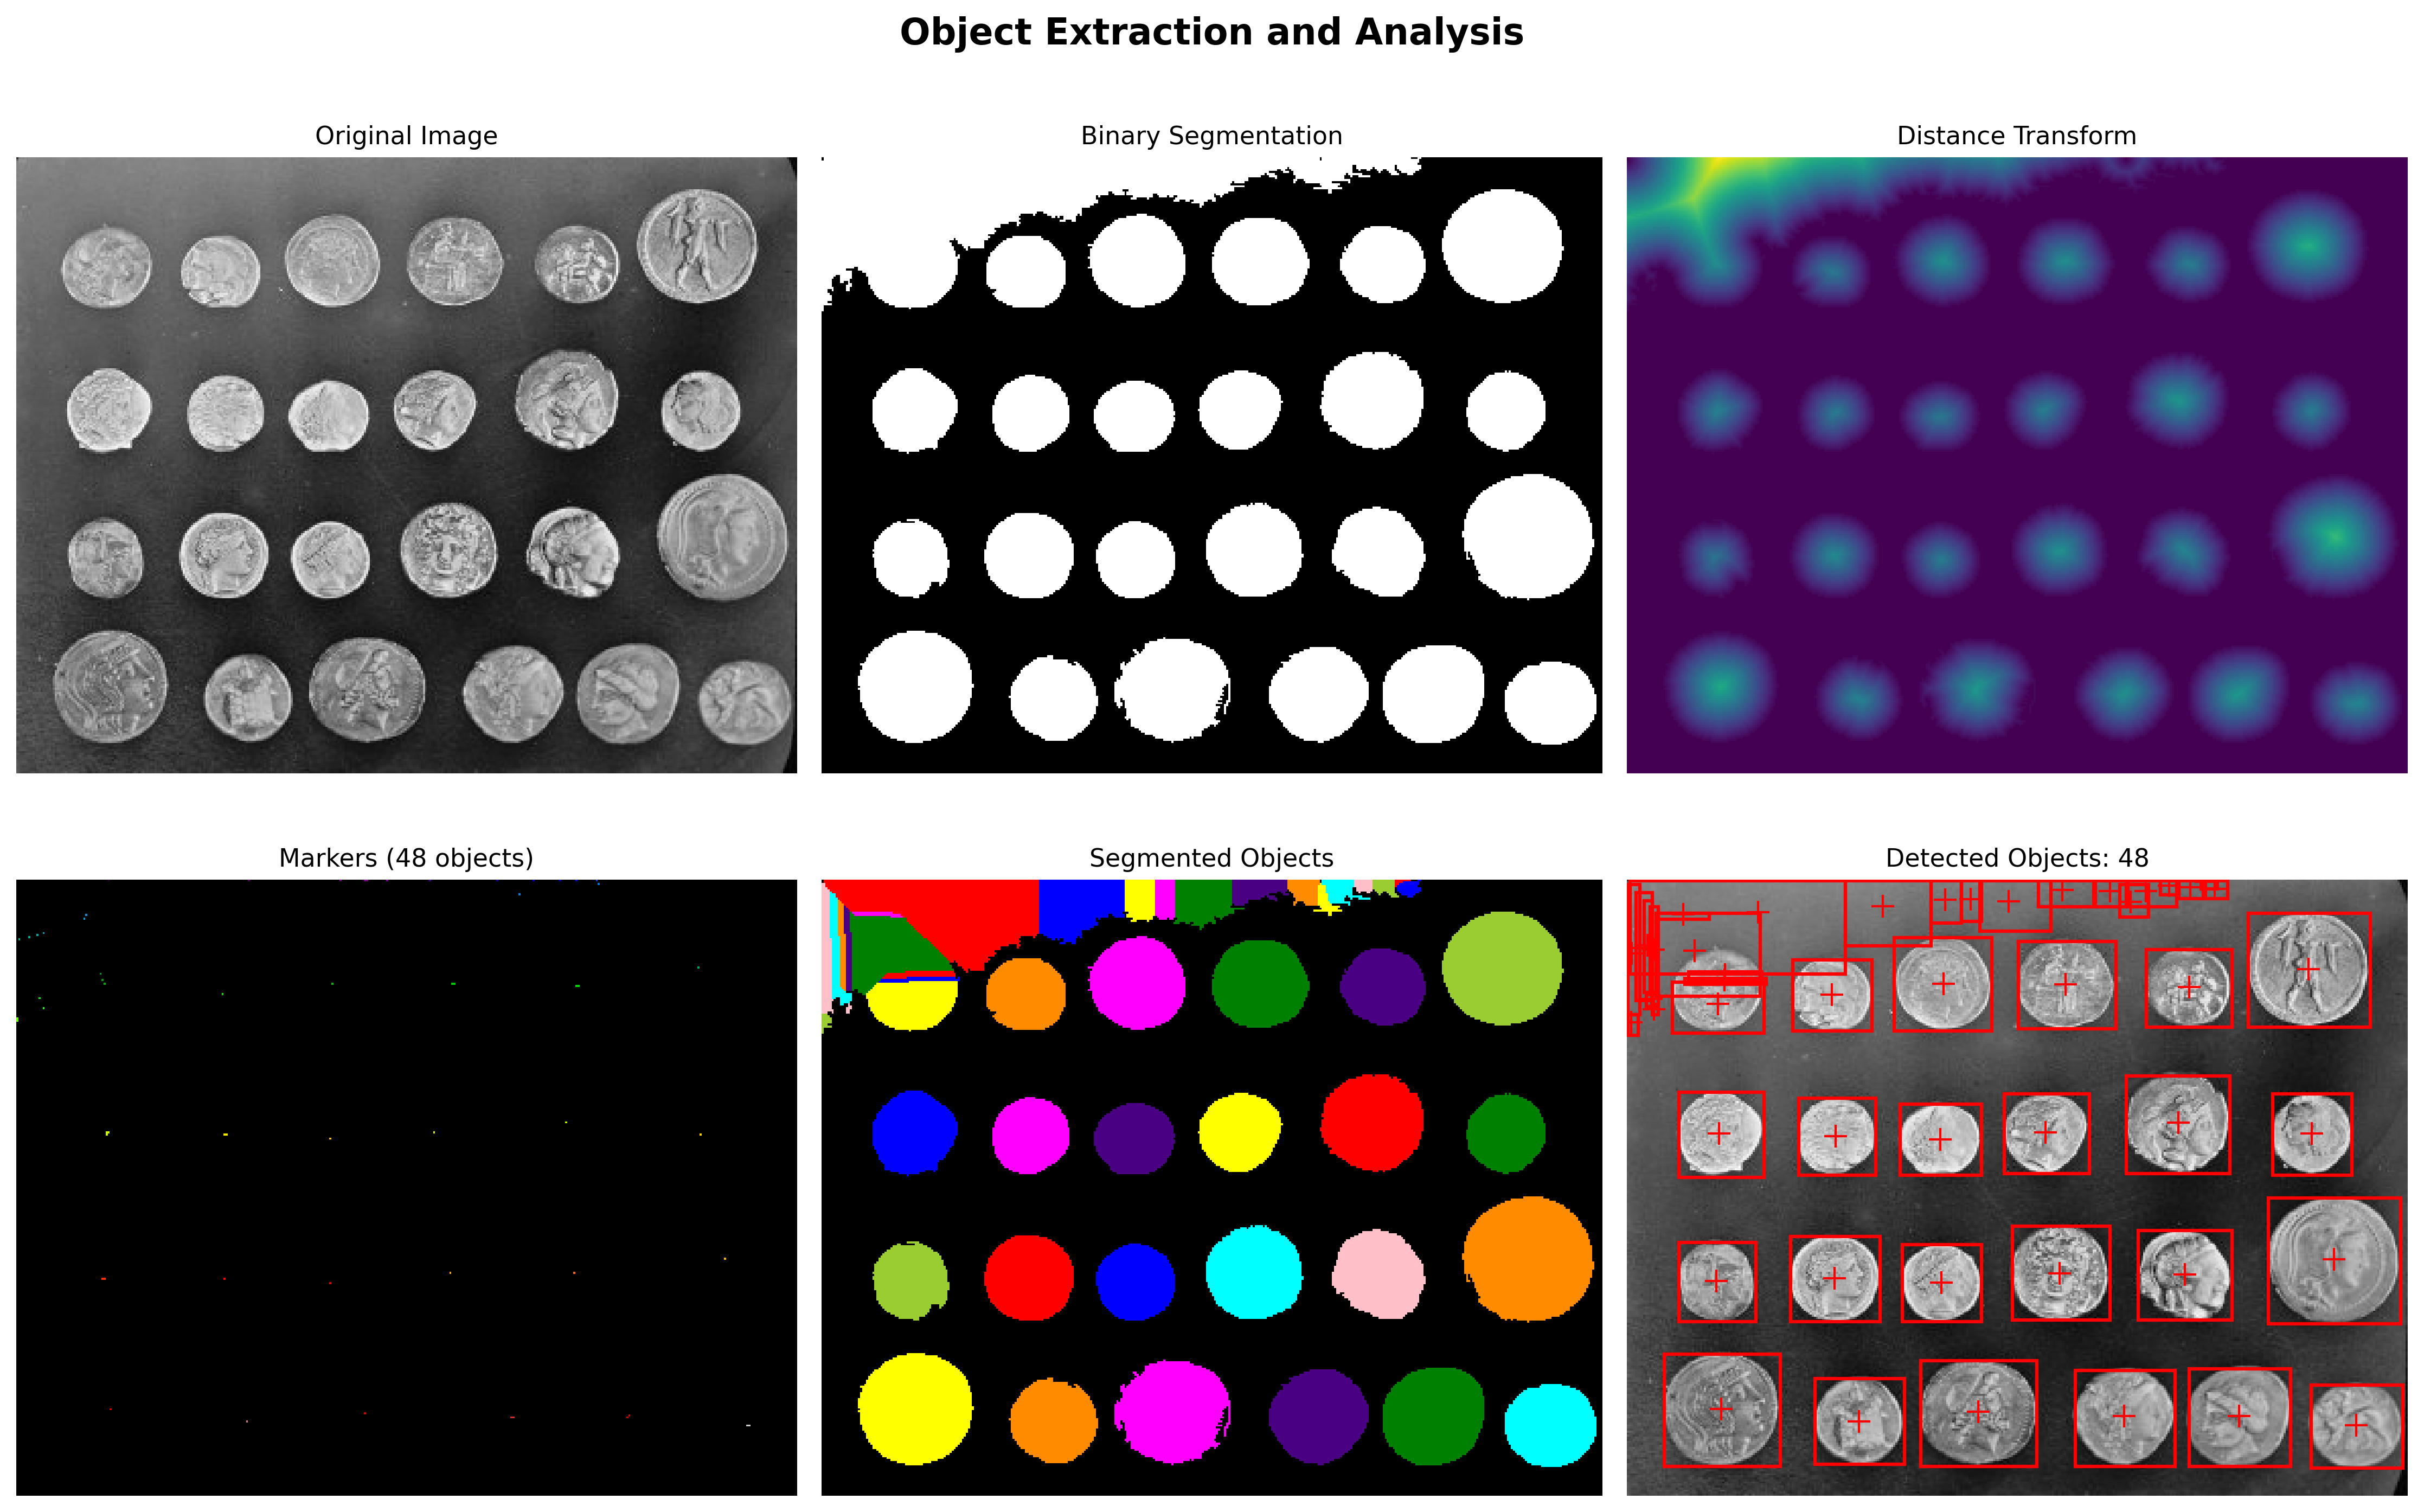
\includegraphics[width=0.92\textwidth,height=0.75\textheight,keepaspectratio]{../figures/13_object_extraction.png}
\end{center}
\end{frame}

\begin{frame}{Texture Enhancement}
\begin{center}
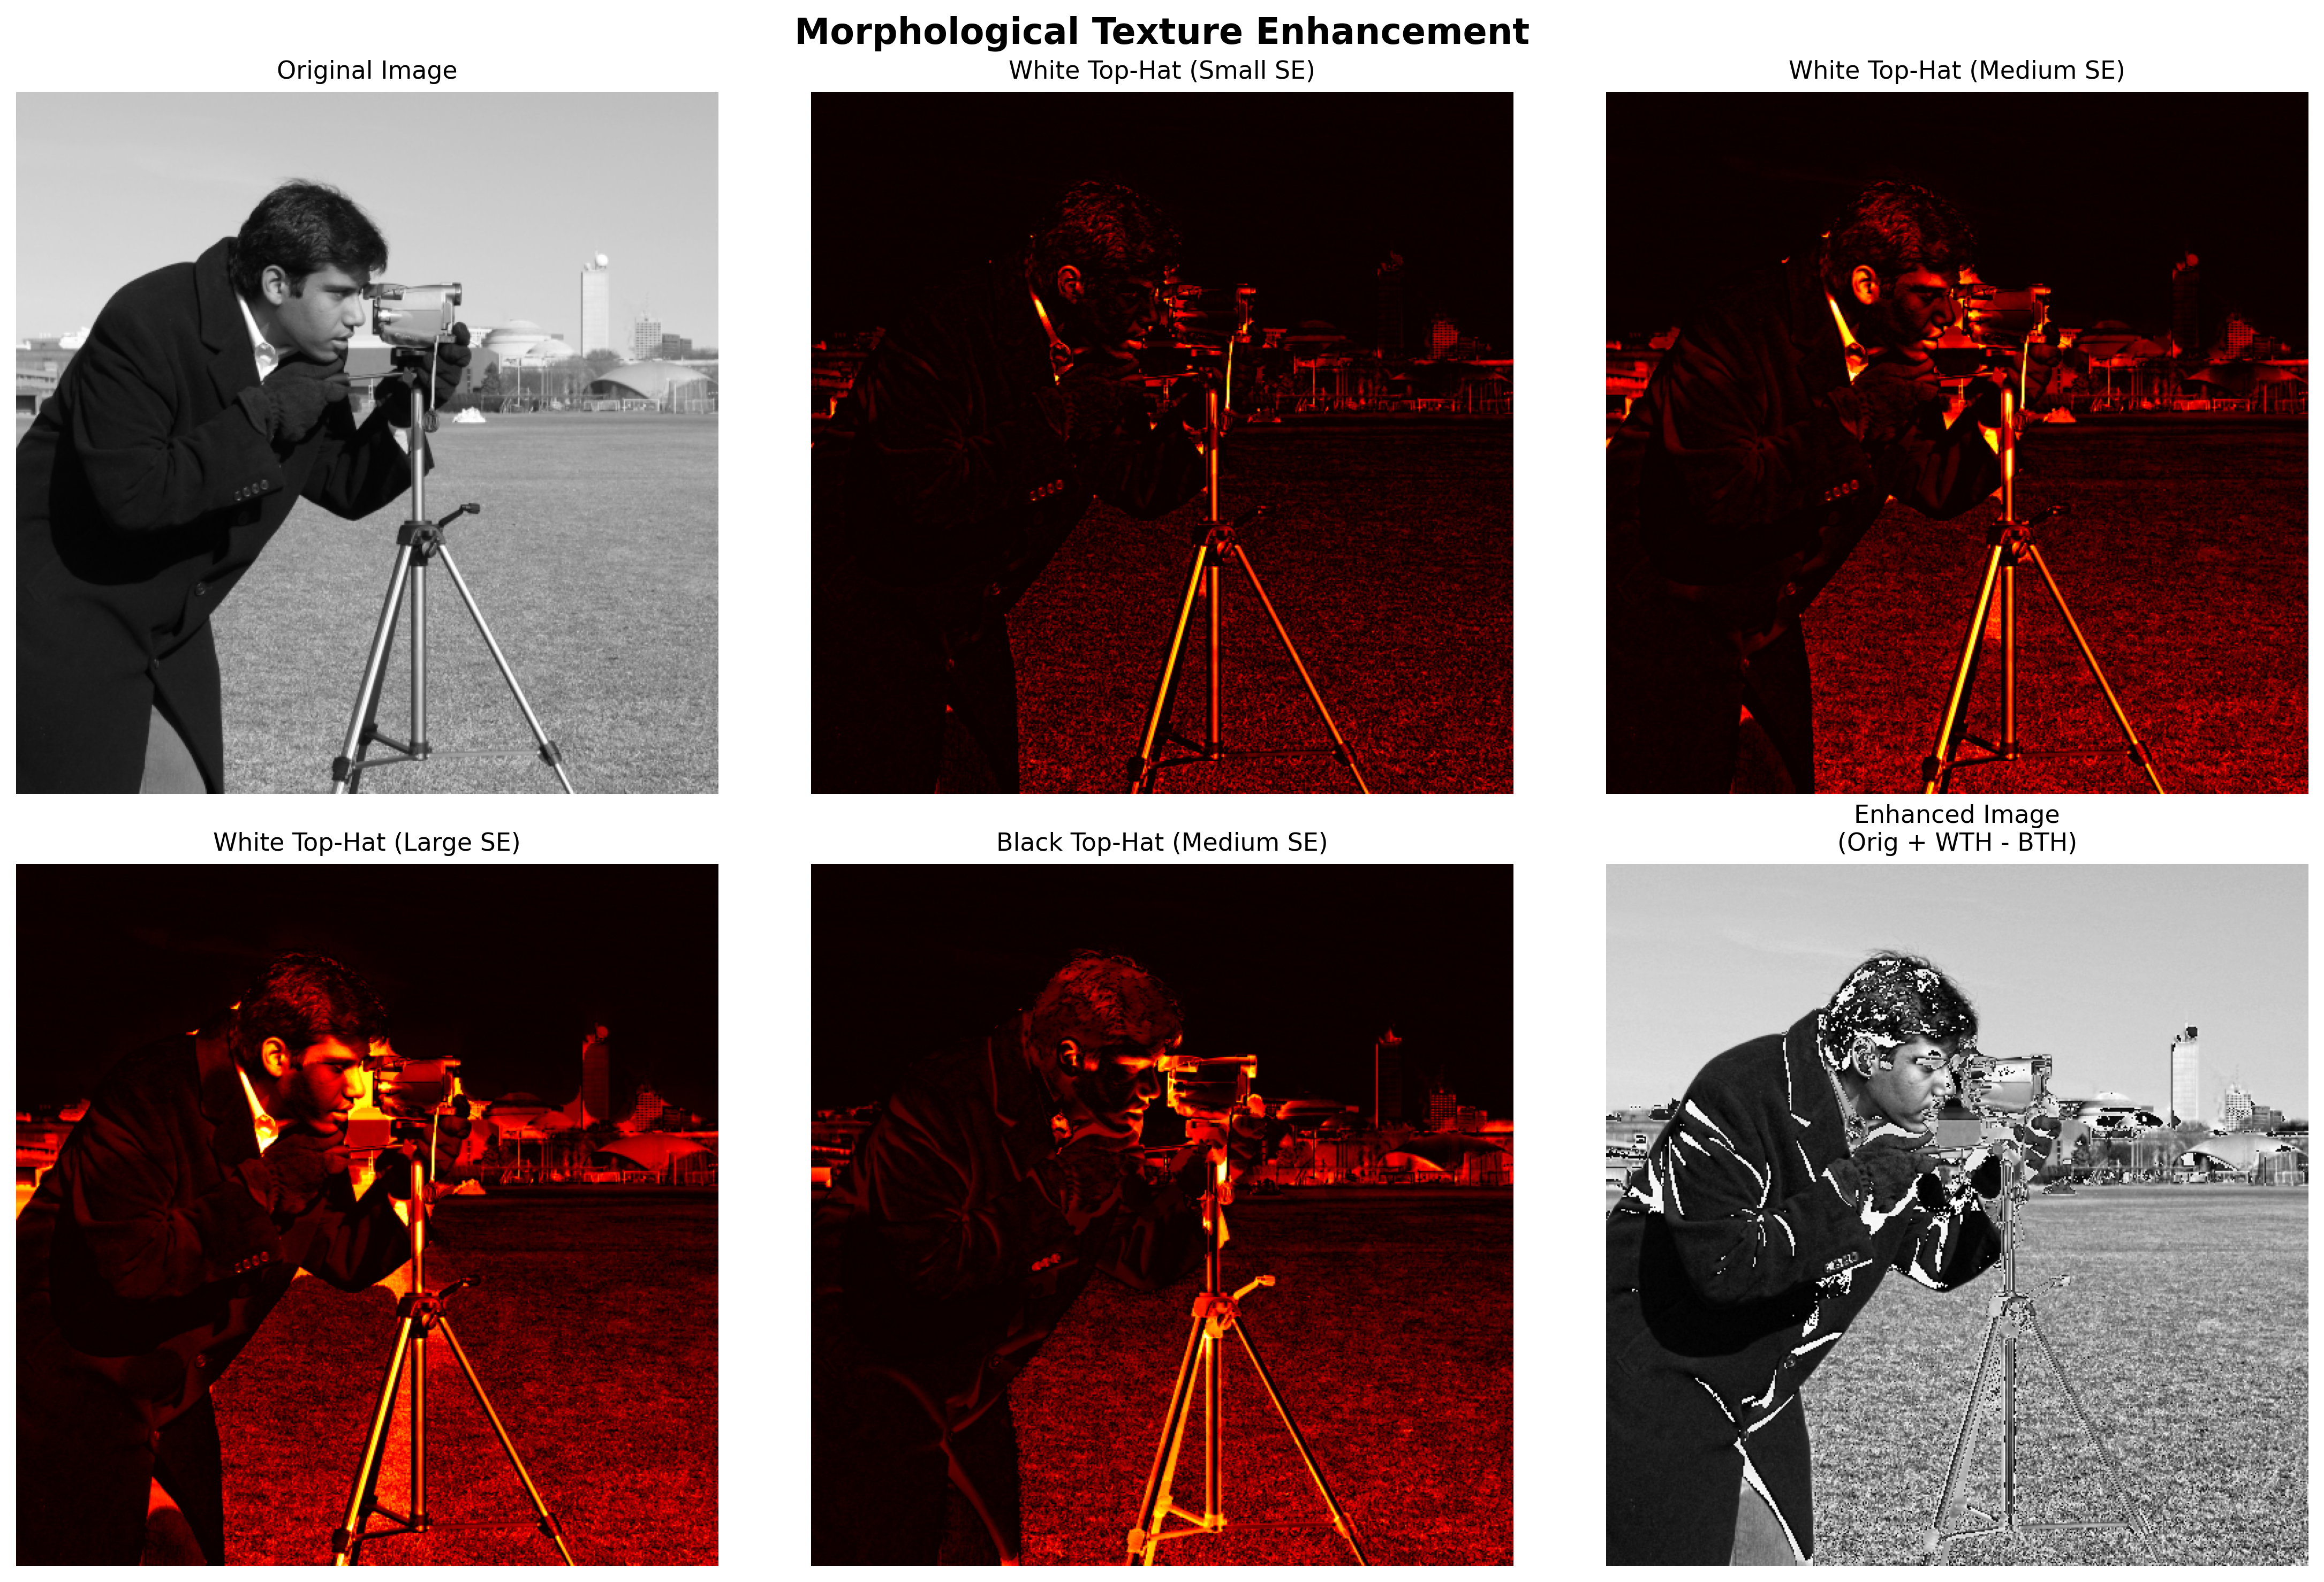
\includegraphics[width=0.9\textwidth,height=0.72\textheight,keepaspectratio]{../figures/14_texture_enhancement.png}
\end{center}
\end{frame}

\begin{frame}{Multi-Scale Segmentation}
\begin{center}
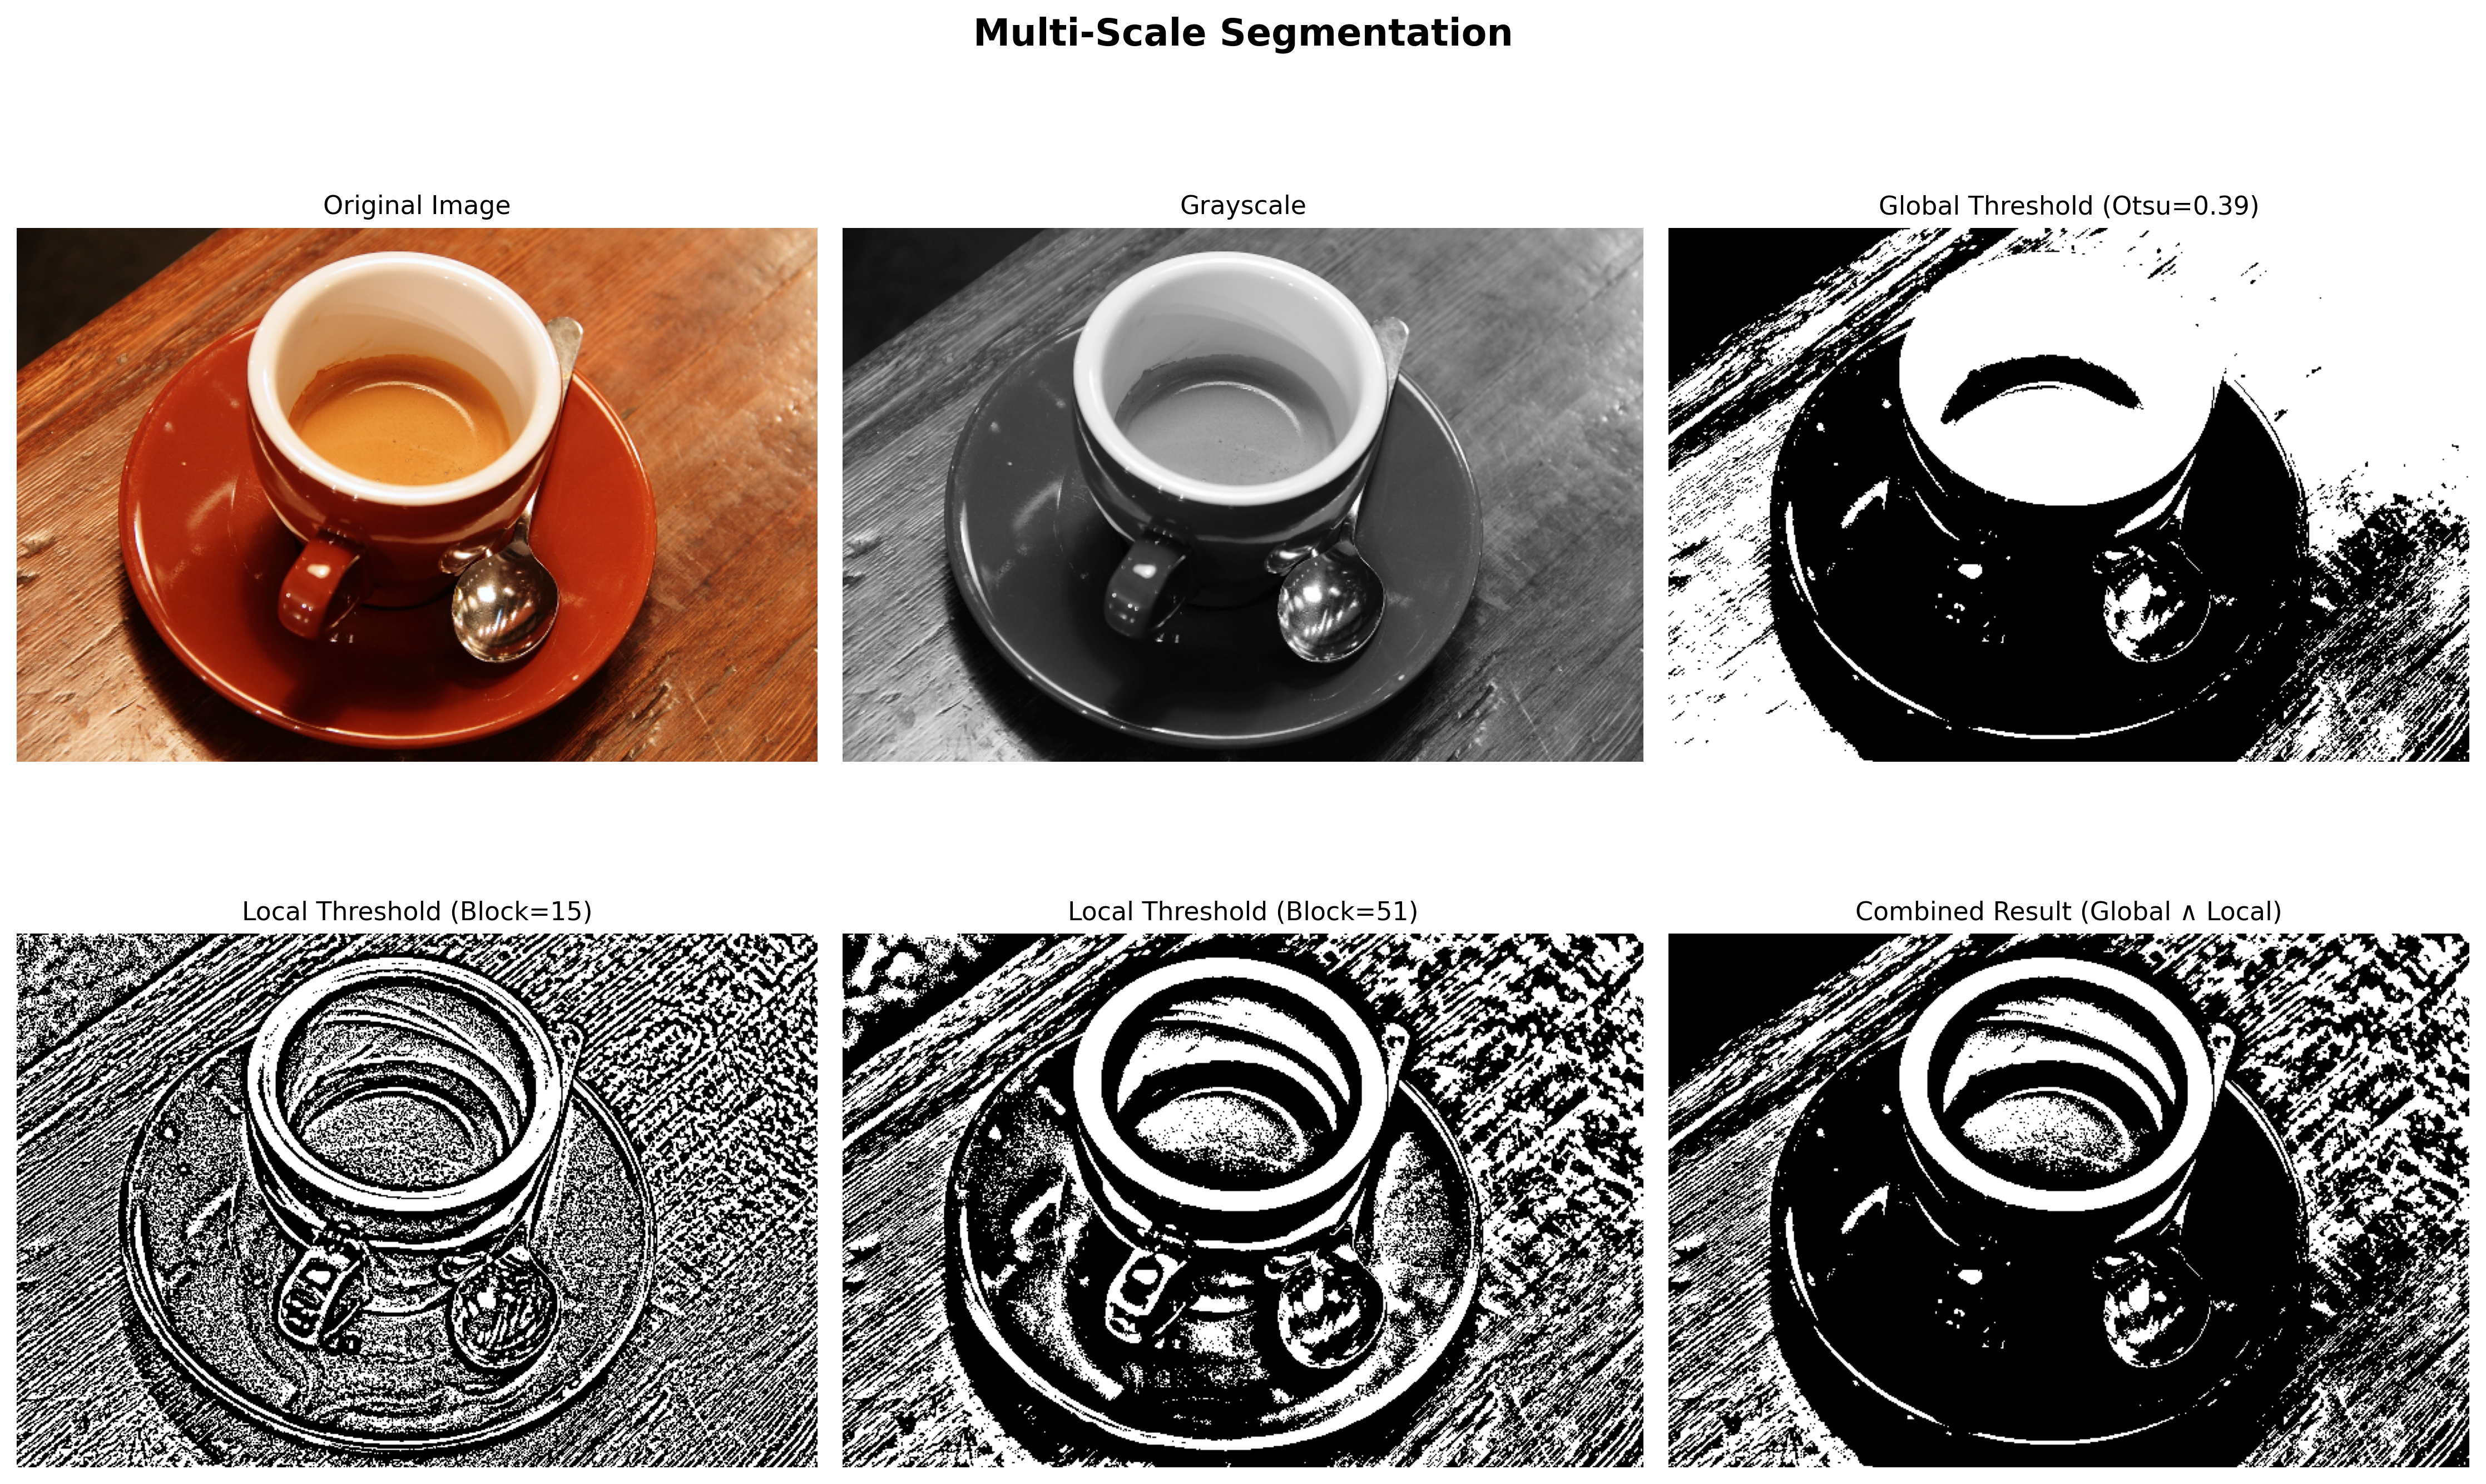
\includegraphics[width=0.92\textwidth,height=0.76\textheight,keepaspectratio]{../figures/15_multi_scale_segmentation.png}
\end{center}
\end{frame}

\section{Best Practices and Guidelines}

\begin{frame}{Choosing Segmentation Methods}
\begin{columns}
\column{0.5\textwidth}
\textbf{Global thresholding:}
\begin{itemize}
\item Uniform illumination
\item Clear bimodal histogram
\item Fast processing required
\end{itemize}

\textbf{Local thresholding:}
\begin{itemize}
\item Non-uniform illumination
\item Gradual intensity changes
\item Document analysis
\end{itemize}

\column{0.5\textwidth}
\textbf{Region-based:}
\begin{itemize}
\item Complex objects
\item Spatial coherence important
\item Interactive segmentation
\end{itemize}

\textbf{Watershed:}
\begin{itemize}
\item Touching objects
\item Known markers available
\item Medical imaging
\end{itemize}
\end{columns}
\end{frame}

\begin{frame}{Structuring Element Selection}
\textbf{Size considerations:}
\begin{itemize}
\item Smaller SE: Preserves fine details, less smoothing
\item Larger SE: Stronger effects, removes more noise
\item Rule of thumb: SE size $\approx$ feature size to remove
\end{itemize}

\textbf{Shape selection:}
\begin{itemize}
\item Disk: Isotropic, general-purpose operations
\item Square: Faster computation, grid-aligned features
\item Custom: Specific directional or shape requirements
\end{itemize}
\end{frame}

\begin{frame}{Common Pitfalls}
\begin{alertblock}{Pitfall 1: Over-segmentation}
Watershed often produces too many regions
\textbf{Solution:} Use marker-controlled watershed or region merging
\end{alertblock}

\begin{alertblock}{Pitfall 2: Threshold sensitivity}
Small changes in threshold drastically affect results
\textbf{Solution:} Use adaptive or multi-threshold methods
\end{alertblock}

\begin{alertblock}{Pitfall 3: Loss of detail}
Morphological operations can over-smooth
\textbf{Solution:} Use smallest effective SE, apply selectively
\end{alertblock}
\end{frame}

\begin{frame}{Parameter Tuning Guidelines}
\textbf{Systematic approach:}
\begin{enumerate}
\item Start with default parameters
\item Visualize intermediate results
\item Adjust one parameter at a time
\item Validate on test images
\item Document optimal settings
\end{enumerate}

\textbf{Validation metrics:}
\begin{itemize}
\item Visual inspection (primary)
\item Region uniformity measures
\item Boundary accuracy
\item Computational efficiency
\end{itemize}
\end{frame}

\section{Summary and Conclusions}

\begin{frame}{Key Takeaways: Segmentation}
\textbf{Thresholding methods:}
\begin{itemize}
\item Simple but powerful for many applications
\item Otsu's method provides automatic threshold selection
\item Local methods handle non-uniform illumination
\end{itemize}

\textbf{Region-based methods:}
\begin{itemize}
\item Region growing: Flexible but seed-dependent
\item Watershed: Effective for separating objects
\item Marker control reduces over-segmentation
\end{itemize}
\end{frame}

\begin{frame}{Key Takeaways: Morphology}
\textbf{Binary morphology:}
\begin{itemize}
\item Erosion and dilation are fundamental operations
\item Opening removes small bright features
\item Closing fills small dark features
\item SE shape and size critical for results
\end{itemize}

\textbf{Grayscale morphology:}
\begin{itemize}
\item Extends binary operations to grayscale
\item Top-hat transforms extract features
\item Morphological gradient for edge detection
\end{itemize}
\end{frame}

\begin{frame}{Integration in Image Processing Pipeline}
\textbf{Typical workflow:}
\begin{enumerate}
\item Preprocessing: Noise reduction, enhancement
\item Segmentation: Threshold or region-based
\item Morphological refinement: Clean and enhance
\item Analysis: Extract features and properties
\item Post-processing: Merge regions, validate
\end{enumerate}

\textbf{Method combination:}
Combining multiple techniques often yields best results
\end{frame}

\begin{frame}{Further Reading and Resources}
\textbf{Classical texts:}
\begin{itemize}
\item Gonzalez \& Woods: Digital Image Processing
\item Soille: Morphological Image Analysis
\item Serra: Image Analysis and Mathematical Morphology
\end{itemize}

\textbf{Modern approaches:}
\begin{itemize}
\item Deep learning segmentation (U-Net, Mask R-CNN)
\item Superpixel methods (SLIC, Felzenszwalb)
\item Graph-based segmentation
\end{itemize}
\end{frame}

\begin{frame}[standout]
Questions?
\end{frame}

\end{document}
